\documentclass{ieeeaccess}
\usepackage{cite}
\usepackage{amsmath,amssymb,amsfonts}
\usepackage{algorithmic}
\usepackage{graphicx}
\usepackage{stfloats}
\usepackage{subfigure}
\usepackage{float}
\usepackage{multirow}
\usepackage{multicol}
\usepackage{enumitem}
\usepackage{xcolor}
\usepackage{romannum}% for approach #1 and #2




\usepackage{textcomp}
\def\BibTeX{{\rm B\kern-.05em{\sc i\kern-.025em b}\kern-.08em
    T\kern-.1667em\lower.7ex\hbox{E}\kern-.125emX}}
\begin{document}
\history{Date of publication xxxx 00, 0000, date of current version xxxx 00, 0000.}
\doi{10.1109/ACCESS.2017.DOI}

\title{DHTCUN: Deep Hybrid Transformer CNN U Network for Single-Image Super-Resolution}
\author{\uppercase{Jagrati Talreja}\authorrefmark{1}, \IEEEmembership{Graduate Student Member, IEEE},
\uppercase{SUPAVADEE ARAMVITH}\authorrefmark{2},\IEEEmembership{Senior Member, IEEE}, AND
\uppercase{Takao Onoye }\authorrefmark{3},
\IEEEmembership{Senior Member, IEEE}}
\address[1]{Department of Electrical Engineering, Faculty of Engineering, Chulalongkorn University, Bangkok 10330, Thailand.}
\address[2]{Multimedia Data Analytics and Processing Unit, Department of Electrical Engineering, Faculty of Engineering, Chulalongkorn University, Bangkok 10330, Thailand.}
\address[3]{Graduate School of Information Science and Technology, Osaka University, 1-5 Yamada-Oka, Suita, 565-0871 Japan}
\tfootnote{This research is funded by the Second Century Fund (C2F), Department of Electrical Engineering, Faculty of Engineering, Chulalongkorn University Bangkok, 10330, Thailand. This research is also funded by Thailand Science Research and Innovation Fund Chulalongkorn University (CU\textunderscore FRB65\textunderscore ind (9)\textunderscore 157\textunderscore 21\textunderscore 23), The NSRF via the Program Management Unit for Human Resources \& Institutional Development, Research and Innovation [grant number B$04G640053$] and also funded by Thailand Science research and Innovation Fund Chulalongkorn University (IND$66210019$). } \markboth
{Author \headeretal: Preparation of Papers for IEEE TRANSACTIONS and JOURNALS}
{Author \headeretal: Preparation of Papers for IEEE TRANSACTIONS and JOURNALS}

\corresp{Corresponding author:  Supavadee Aramvith (supavadee.a@chula.ac.th).}

\begin{abstract}
Recent advances in image super-resolution have investigated various transformer and CNN techniques to improve quantitative and perceptual outcomes. Reconstructing high-resolution images from their low-resolution equivalents by combining the power of transformers and CNN has been a crucial task in recent times. We propose a novel U-shaped architecture that integrates transformers and convolutional neural networks (CNNs) to leverage the strengths of both approaches. The network incorporates a novel Parallel Hybrid Transformer CNN Block (PHTCB) on the backbone of the U-shaped design, ensuring computational efficiency and robust hierarchical feature representation. Our architecture incorporates triple enhanced spatial-attention mechanisms, and a Transformer CNN (TCN) Block in PHTCB. The TCN Block helps preserving sharp edges and intricate details that are often lost in traditional SISR methods and enhances the visual fidelity of the reconstructed high-resolution images. Additionally, we introduce the triple-enhanced spatial attention (TESA) approach that helps in precise localization of important features. By focusing on these critical areas, blurring can be reduced for crucial features because of the network's ability to control features at various scales. Experiments demonstrate that our proposed method yields better quantitative measurements, including visually appealing high-resolution image reconstructions, peak signal-to-noise ratio (PSNR), and structural similarity index (SSIM).
\end{abstract}

\begin{keywords}
CNN; Enhanced Spatial Attention; Single-Image super-resolution; Transformer. 
\end{keywords}

\titlepgskip=-15pt

\maketitle

\section{Introduction}
\label{sec:introduction}
\PARstart{I}n the rapidly evolving field of image processing and computer vision, the pursuit of high-fidelity image super-resolution (SISR) stands as a cornerstone challenge. The primary goal of SISR is to reconstruct high-resolution images from their low-resolution counterparts, a task that holds significant importance across a multitude of applications, including medical imaging [1], satellite imagery analysis [2], surveillance [3], and multimedia enhancement [4]. Recent years have seen a surge in research focused on improving both the quantitative metrics and perceptual quality of super-resolved images. Central to these advancements is the synergistic integration of transformer models and convolutional neural networks (CNNs), leveraging the unique strengths of each to achieve superior results.

Due to the creation of numerous High-Resolution (HR) images that correspond to a single Low-Resolution (LR) image, SISR is an ill-posed problem. In recent years, single image super-resolution (SISR) has seen remarkable advancements, with convolutional neural networks (CNNs) emerging as the dominant approach. These CNN-based models have significantly improved the quality of generated high-resolution (HR) images, making them the mainstream method for SISR tasks. The advent of convolutional neural networks (CNNs) was pioneered in Super-Resolution Convolutional Neural Networks (SRCNN) [5],  by Dong et al. Following the SRCNN approach, researchers have delved into various aspects of image super-resolution, including model frameworks, up-sampling methods, network design, and learning strategies in models like FSRCNN [6], VDSR [7], LapSRN [8], MemNet [9], EDSR [10], RCAN [11], NLSN [12] and DANS [13]. This exploration has yielded a variety of sophisticated techniques aimed at enhancing the performance and efficiency of SISR models. However, despite their success, CNN-based models encounter several limitations, including constrained receptive field, introduction of blurring, jagged patterns or over-smoothing. These limitations hinder their efficiency and scalability, especially when dealing with large and complex images.

On the other hand, Vision Transformers (ViTs) [14] have demonstrated superior modeling capabilities and a larger receptive field, enabling them to capture long-range dependencies and global context more effectively than CNNs. ViTs leverage the self-attention mechanism to process the entire image as a sequence of patches, allowing them to model relationships between distant pixels and capture holistic image features. The self-attention mechanism in Transformers, while powerful, is computationally expensive, especially as the resolution of the input image increases. This high resource demand can be prohibitive for practical applications, particularly in environments where computational efficiency and memory usage are critical considerations. The introduction of ViT led to several advancements and modifications to address the challenges associated with applying Transformers to SISR such as Swin IR [15], Swin Transformer [16] SRFormer [17], ELAN [18], TCDFN [19], and HNCT [20]. However, the application of Transformers to SISR tasks comes with its own set of challenges. Notably, Transformers require extensive computing power and memory, which can be prohibitive for practical applications. The high resource demands of Transformers limit their widespread adoption in scenarios where computational efficiency and memory usage are critical considerations.

Given the current trend towards fast processing devices minimizing model size is crucial for achieving rapid and state-of-the-art (SOTA) comparable results for higher scale factors. Although CNN as well as transformers have greatly succeeded to enhance network performance, they still encounter certain limitations.

(1) Sometimes, these methods can introduce distortions into super-resolved images such as jagged patterns, blurring or over-smoothing in extremely textured regions.

(2) The previously mentioned techniques require significant processing power and time, and they are computationally expensive. Moreover, processing large datasets or high-resolution images further exacerbates the computational burden, potentially leading to longer processing times and reduced real-time performance.

(3) In some cases, attempts to enhance image resolution may inadvertently amplify noise or artifacts, resulting in degraded image quality and increased visual distortion. As a consequence, achieving satisfactory super-resolution outcomes for extremely low-resolution and noisy input images remains a significant challenge in the field of image processing.

One way to efficiently address these challenges is to merge the complementary abilities of CNNs and Transformers and integrate their strengths. Transformers have been proven to capture long-range dependencies effectively where as the CNNs advance in enhanceing the quality of noisy images without compromising the computational expense. Some of the Hybrid models have already been proposed such as EHNet [21], HNCT [20], and TCDFN [19]. Utilizing comparable methodologies, we put forth a unique strategy for single-image super-resolution that combines the CNN and Transformer in a U-shaped architecture with skip connections. The U shaped design with skip connections acts as the backbone of our proposed method and helps the network to extract features differently from different layers without increasing the combutational burden. The transformer helps to capture long range dependencies and global context and reduce the artifactes like jagged patterns or blurring. The CNN help in better enhancing the quality of noisy images and prevent the amplification of noise during restoration of noisy images. This synergetic combination allows the model to enhance the super-resolution performance while reducing its compuattional burden.

The following is a summary of the primary contributions made by our suggested model:

(i)	Propose a Parallel Hybrid Transformer CNN Block (PHTCB) having a Transformer CNN (TCN) Block which combines the powers of CNNS and Transformer to capture long range dependencies, reduce artifacts and simultaneously prevents the amplification of noise in super-resolution of noisy images.

(ii)	Put forth a Triple Enhanced Spatial Attention (TESA) block to improve the performance of the model by focusing on relevant image regions while suppressing irrelevant or noisy areas.

(iii)	Suggest a U-shaped backbone with skip connection to extract features differently from different layers without increasing the combutational burden.

The article's remaining sections are Section II, which examines relevant research on the suggested approach, and Section III, which outlines the network's methodology. The experimental results and a comparative analysis using cutting-edge techniques are presented in Section IV. Sections V and VI contain a discussion and conclusion along with suggestions for further work.

\section{RELATED WORK}
Throughout the past ten years, the field of image super-resolution (ISR) has made great strides, mostly due to the development of various deep learning algorithms. Convolutional neural networks (CNNs), generative adversarial networks (GANs), attention mechanisms, and transformer-based models are some of the major categories into which these developments can be divided.

The foundation of many advances in ISR has been Convolutional Neural Networks (CNNs). A major turning point in the discipline was reached when Dong et al. introduced SRCNN [5], showcasing deep learning's potential for super-resolution applications. In order to improve performance, later efforts have concentrated on strengthening CNNs' architecture and training methodologies. A significant contribution in this domain is the Fast Super-Resolution Convolutional Neural Network (FSRCNN) [6] by Dong et al. FSRCNN [6] was designed to be a faster and more efficient model than its predecessors. LapSRN [8] developed by Lai \textit{et al}. uses a progressive reconstruction approach via a pyramid of images, improving both training and testing efficiency. A Memory persistant network MemNet [9] was introcuded by Tai \textit{et al}. to better handle the memory requirements of the network. Li \textit{et al}. proposed the Super-Resolution Feedback Network (SRFBN) [22], which uses feedback connections to refine feature representations iteratively, resulting in enhanced super-resolution quality. To get better results, Kim \textit{et al}., for example, proposed the VDSR [7] model, which used an extremely deeper CNN layers and residual learning to enhance super-resolution performance. Deeply-Recursive Convolutional Network (DRCN) [23] and Deeply-Recursive Residual Network (DRRN) [24] by Kim \textit{et al}. leverage recursive learning to improve depth and performance with fewer parameters. As deeper networks were not suitable ofr the currect cutting edge devices, by deleting pointless modules from conventional CNNs, the EDSR [10] model by Lim \textit{et al}. stretched the envelope even farther and produced a more potent and effective network by improving optimization strategy and winning the New Trends in Image Restoration and Enhancement (NTIRE) 2017 challenge on single image Super-Resolution: Dataset and Study. To handle multiple scale factors in a single model Multi-Scale Deep Cross Network for Image Super-Resolution (MDCN) [25] was introduced. 
To further improve the visual quality, Generative Adversarial Networks (GANs) introduced a new paradigm in ISR by focusing on generating more realistic and perceptually pleasing images. Ledig \textit{et al}. introduced SRGAN [26], that utilized GANs for ISR, producing high-resolution images with sharper details. Subsequent models, such as ESRGAN [27] by Wang \textit{et al}., improved upon SRGAN by incorporating a deeper and more complex generator and discriminator architecture, furthermore EnhanceNet [28] was also introduced which led to further enhancements in image quality.

Attention mechanisms have been pivotal in enhancing feature representation in ISR models. The integration of attention mechanisms into ISR models has significantly improved their ability to focus on important features of the image. The work by Zhang \textit{et al}. on the Residual Channel Attention Network (RCAN) [11] demonstrated the effectiveness of channel attention mechanisms in enhancing feature representation. Similarly, Dai \textit{et al}. proposed the Second-order Attention Network (SAN) [29], which leverages second-order channel attention to capture more complex feature interactions. Cross-Scale Non-Local (CSNL) [30] attention network by Mei et al, which captures dependencies across different scales to enhance the representation of complex image structures. The Holistic Attention Network (HAN) [31] by Niu et al. integrates both spatial and channel-wise attention mechanisms at multiple levels of the network to effectively capture fine-grained details. MFCC [32], which leverages multi-frequency information through channel attention, improving the network's ability to distinguish between different textures and details in the image. Mei et al. developed the Non-Local Sparse Attention Network (NLSN) [12], which uses non-local operations to capture long-range dependencies and sparse attention mechanisms to reduce computational complexity while maintaining performance. These advancements have shown that attention mechanisms can significantly boost the performance of CNN-based ISR models by allowing them to dynamically adjust their focus based on the input image. DANS [13] refine feature maps at various stages of the network, significantly enhancing the quality of super-resolved images and SENext [33] by W. Muhammad \textit{et al}. incorporates advanced channel-wise attention mechanisms to recalibrate feature responses dynamically, improving super-resolution performance while simultaneously reducing computational cost and prevents over-fitting. But careful consideration and investigation of these issues are still required.

Enhanced spatial attention mechanisms have been explored to improve the performance of ISR models. Woo et al. introduced the Convolutional Block Attention Module (CBAM) [34], which combines spatial and channel attention mechanisms to refine feature representations. This approach has been shown to effectively enhance image quality by allowing the model to focus on relevant regions and suppress noise. Similarly, the dual attention mechanism proposed by Zhang et al. in the DANet [35] model demonstrated the benefits of incorporating both spatial and channel attention for image super-resolution tasks.


\begin{figure}

    \centering
    \newlength{\xfigwd}
    \subfigure {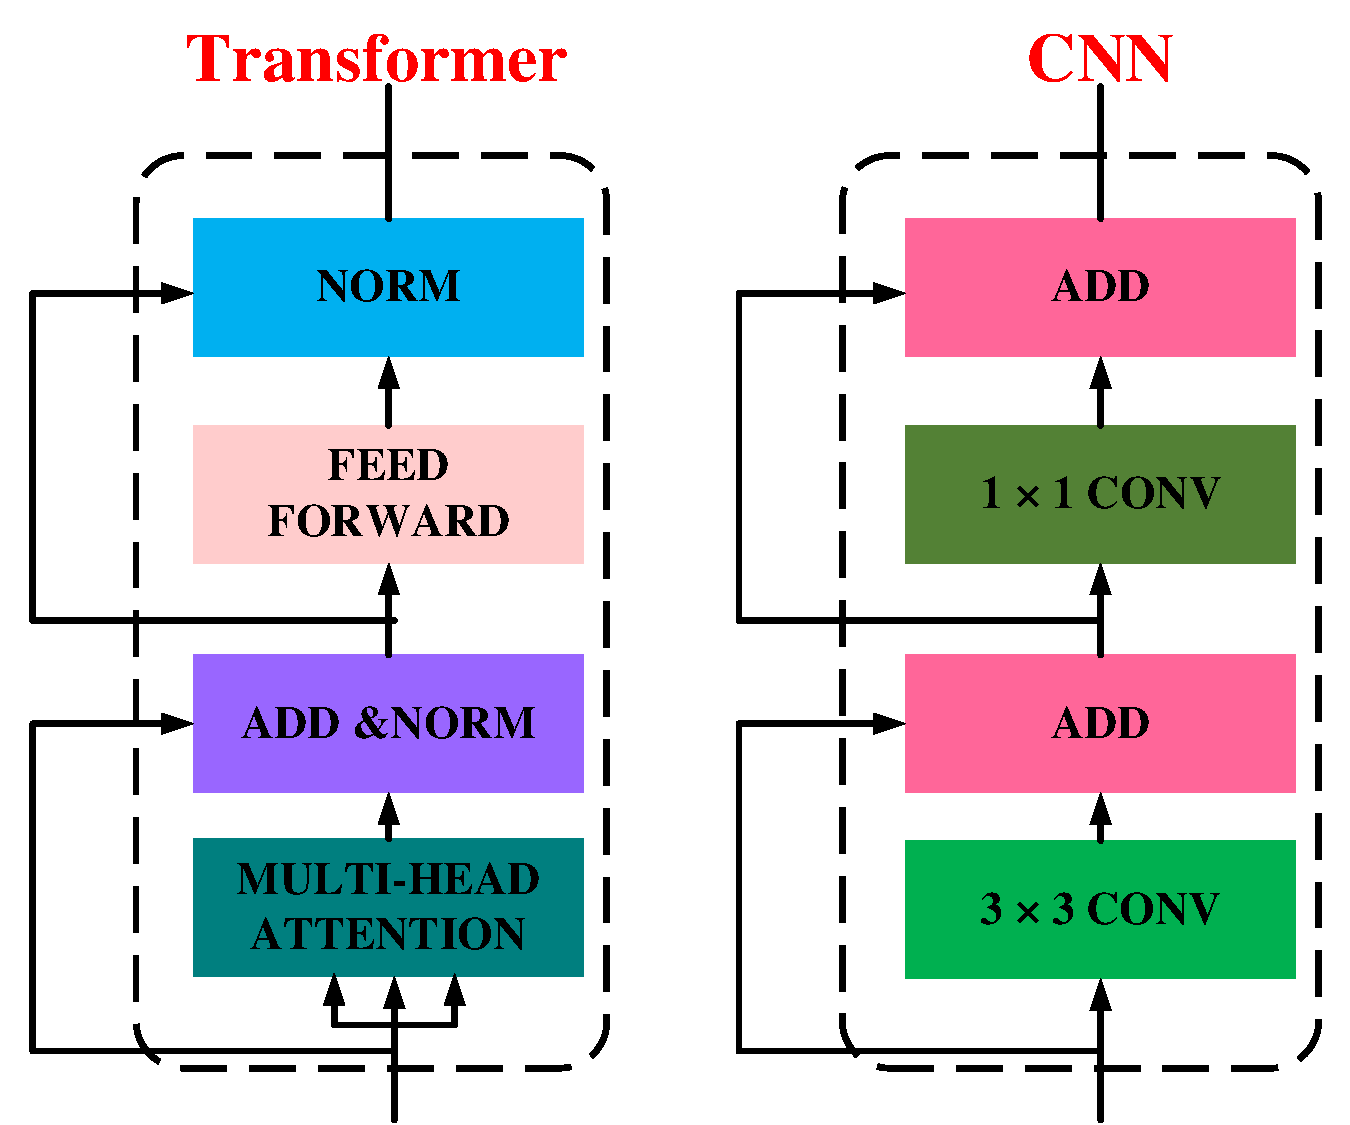
\includegraphics[width=\linewidth]{1FIGURE.pdf}}
    \caption {General Architecture of Transformer and CNN networks.}

    \label{fig1}
\end{figure}

Recently, transformer-based models have gained popularity in ISR due to their capability to capture long-range dependencies and model global context more effectively than CNNs. Vision Transformers (ViTs) [14], introduced by Dosovitskiy et al., demonstrated the potential of transformers in various vision tasks. The Swin Transformer by Liu et al [16]. proposed a hierarchical transformer model with shifted windows, which significantly reduced computational complexity while maintaining high performance. Liang et al. introduced the SwinIR [15] model, which integrated the Swin Transformer into a residual network, showcasing its effectiveness in image restoration tasks. ELAN [18] architecture is designed to harness the power of long-range attention mechanisms while maintaining computational efficiency. SRFormer [17] introduces multi-head self-attention mechanisms to capture complex relationships between distant pixels, improving the network's ability to reconstruct fine details and textures in the super-resolved images. SRFormer incorporates positional encoding, which helps the model understand the relative positions of pixels, enhancing its spatial awareness. 
Hybrid models combining the strengths of CNNs and transformers have been proposed to leverage both local feature extraction and global context modeling. For instance, the TransCNN [36] model by Waseem et al. combined CNN and transformer blocks to achieve state-of-the-art results in ISR. The IPT [37] model by Chen et al. used a large-scale pre-trained transformer for various image processing tasks, including ISR, HNCT [20] and TCDFN [19] are also some of the hybrid approaches highlighting the versatility and power of transformer-based approaches.

The landscape of image super-resolution has been significantly enriched by advancements in CNNs, GANs, attention mechanisms, transformer-based models, hybrid approaches, and efficient model design. Each of these techniques has contributed to improving the quality and performance of ISR models, addressing various challenges such as computational complexity, memory requirements, and the need for real-time processing on edge devices. The ongoing research and development in these areas continue to push the boundaries of what is possible in image super-resolution, paving the way for more sophisticated and practical applications. In this work, a novel approach to U-Shaped network architecture combining CNN and transformer is laid out. The goal of bringing together these parts is to further improve image super-resolution performance by utilizing the advantages of both transformers and CNNs.

To sum up, advances in image super-resolution have been made possible by deep learning-based methods, CNNs, transformers, and network designs. By combining these methods, reconstruction quality has significantly improved, allowing for the creation of more detailed high-resolution images. Research issues include adapting SR approaches to video super-resolution, generalizing across domains, and maximizing computational efficiency. These developments are needed to realize the full potential of image super-resolution in various applications, including digital content creation [38], medical imaging [1], surveillance [3], remote sensing [39], and facial image super-resolution [40].


\begin{figure*}
    \centering

    \includegraphics[width=\linewidth]{2Figure.pdf}
    \caption{Deep Hybrid Transformer CNN U-Net for Single Image Super Resolution's (DHTCUN) proposed network architecture.}
    \label{fig:1}
\end{figure*}

\section{PROPOSED METHODOLOGY}

This section presents our proposed novel hybrid approach in single image super-resolution by fusion of Transformer and CNN in a Parallel Hybrid Transformer CNN Block (PHTCB) in a U-shaped design framework. Furthermore, we employed the enhanced spatial attention in the network architecture to refine feature representations and allows the model to focus on relevant regions and suppress noise. Moreover, the information from PHTCB is transfered using skip connections to transmit low-frequency information at each stage of the network to reduce the parameters for the computation. Finally, we use pixel shuffle for reconstructing the high resolution image.

Figure 2 shows, our proposed Deep Hybrid transformer U-Network for Single Image Super-Resolution (DHTCUN) consisting of five Parallel Hybrid Transformer CNN Blocks (PHTCB) described in the section 3A. The initial low-resolution feaatures are extracted using a normal convolution 1 $\times$ 1. Then the features are transmitted in the U shaped architecture designed using the PHTCB. The less complex features are directly transmitted from the first PHTCB to the last PHTCB using a skip connection where the more complex featurex features traverse through second PHTCB to the second-last PHTCB. The higher the complexity of the feature, the more they traverse through the PHTCB to ayttain better refinement. These features after passing from the U-shaped framework, pass through the Enhanced spatial attention block followed by a 1 $\times$ 1 convolution layer to achieve better refinement  by focusing on the relevant features and and noise suppression. Finally, the High-resolution image is recunstructed using a Pixel Shuffle folowed by two layers of the 3 $\times$ 3 convolution.

The initial features extraction is indicated in Equation 1.

\begin{equation}
{H_{0}}= {F_{Conv1}}({H_{LR}}),
\end{equation}

Here, ${H_{LR}}$ is the input Low-Resolution (LR) image, ${F_{Conv1}}$$(.)$ represents 1 $\times$ 1 convolution operation for extracting initial features, and ${H_{0}}$ is the output of the convolution layer. 

After passing through the initial feature extraction stage, the features are transmitted to the PHTCB in the U-shaped framework.


\subsection{Parallel Hybrid Transformer CNN Block (PHTCB)}

Parallel Hybrid Transformer CNN Block (PHTCB) is used to capture long range dependencies, reduce artifacts and simultaneously prevents the amplification of noise in super-resolution of noisy images. The architecture of PHTCB is shown in Figure 3. It consist of Triple Enhanced Spatial Attention (TESA) described in section 3 A.1 Block and Transformer CNN (TCN) Blocks described in section 3 A.2. Since the hybrid combination of Transformer and CNN is parallely connected in this block, that's why the Block is named as Parallel Hybrid Transformer CNN Block (PHTCB). 

As seen in Figure 3, the PHTCB consist of the TESA and the TCN Blocks. The input to the PHTCB first passess through the TESA and then is parallely distributed through both the Hybrid TCN Blocks. The TCN block is the Hybrid block cascading together the Swin Transfromer Layer (STL) and the convolutional layer. Finally the features pass through a covolutional layer and passed through a TESA followed by an arithmetic addition.

The mathematical expression of PHTCB is given in Equation 2, 3, 4, 5 and 6.

The input to the PHTCB is fed to the TESA block. The euation of the TESA Block is given by Equation 2.

\begin{equation}
{H_{TESA}}= {F_{TESA}}({H_{I}}),
\end{equation}

Here, ${H_{I}}$ is the input to the PHTCB block,  ${F_{TESA}}$$(.)$ is the TESA Block function and ${H_{TESA}}$ is the output of the TESA block.

The output of the TESA block is distributed parallely to the TCN blocks. The output of each TCN block is shown by Equation 3.

\begin{equation}
\begin{aligned}
    {H_{TCN}} &= \bigl(F_{\text{STL}}(F_{\text{Conv3}}(H_{\text{TESA}}))\bigr) \\
   % &\quad+ \bigl(F_{\text{STL}}(F_{\text{Conv3}}(H_{\text{TESA}}))\bigr),
\end{aligned}
\end{equation}

Here, ${F_{\text{Conv3}}}$$(.)$ is the 3 $\times$ 3 convolution function, ${F_{\text{STL}}}$$(.)$ is the STL function and ${H_{TCN}}$ is the output of the TCN block

The outputs of both the TCN blocks are added and passed through th convolution layer in Equation 4 and 5.

\begin{equation}
{H_{Con_{i/p}}}= {H_{TCN1}} + {H_{TCN2}},
\end{equation}

Here, ${H_{Con_{i/p}}}$ is the input to the 1 $\times$ 1 convolution layer, ${H_{TCN1}}$ and ${H_{TCN2}}$ are the outputs from both the TCN block. ${H_{TCN1}}$ = ${H_{TCN2}}$ = ${H_{TCN}}$

\begin{equation}
{H_{Con_{o/p}}}= {F_{Conv1}}({H_{Con_{i/p}}}),
\end{equation}

Here, ${H_{Con_{o/p}}}$ is the output of the 1 $\times$ 1 convolution layer and ${F_{Conv1}}$$(.)$ represents 1 $\times$ 1 convolution operation.

Finally, all the features are passed through the TESA block.

\begin{equation}
{H_{PHTCB}}= {F_{TESA}}({H_{Con_{o/p}}}),
\end{equation}

Here ${H_{PHTCB}}$ denotes the ouput of the PHTCB block


\subsubsection{Triple Enhanced Spatial Attention (TESA) Block}

The Triple enhannce Spatial Attention as seen in Figure 4, consists of three Enhanced Spatial Attention (ESA) modules stacked together. This approach enhances image quality by focusing on relevant regions of the image. TESA employs an iterative approach where the output of one attention module is refined by subsequent modules, progressively enhancing the focus on critical features.The output of TESA is shown by Equation 7.

\begin{equation}
{H_{TESA}}= {F_{ESA}}({F_{ESA}}({F_{ESA}}({H_{i/p}}))),
\end{equation}

Here ${F_{ESA}}$$(.)$ represents the Enhanced Spatial Attention (ESA) module, and $({H_{i/p}})$ is the input fed into the TESA block and  ${H_{TESA}}$ is the output of the TESA Block.

\begin{figure}[ht]
  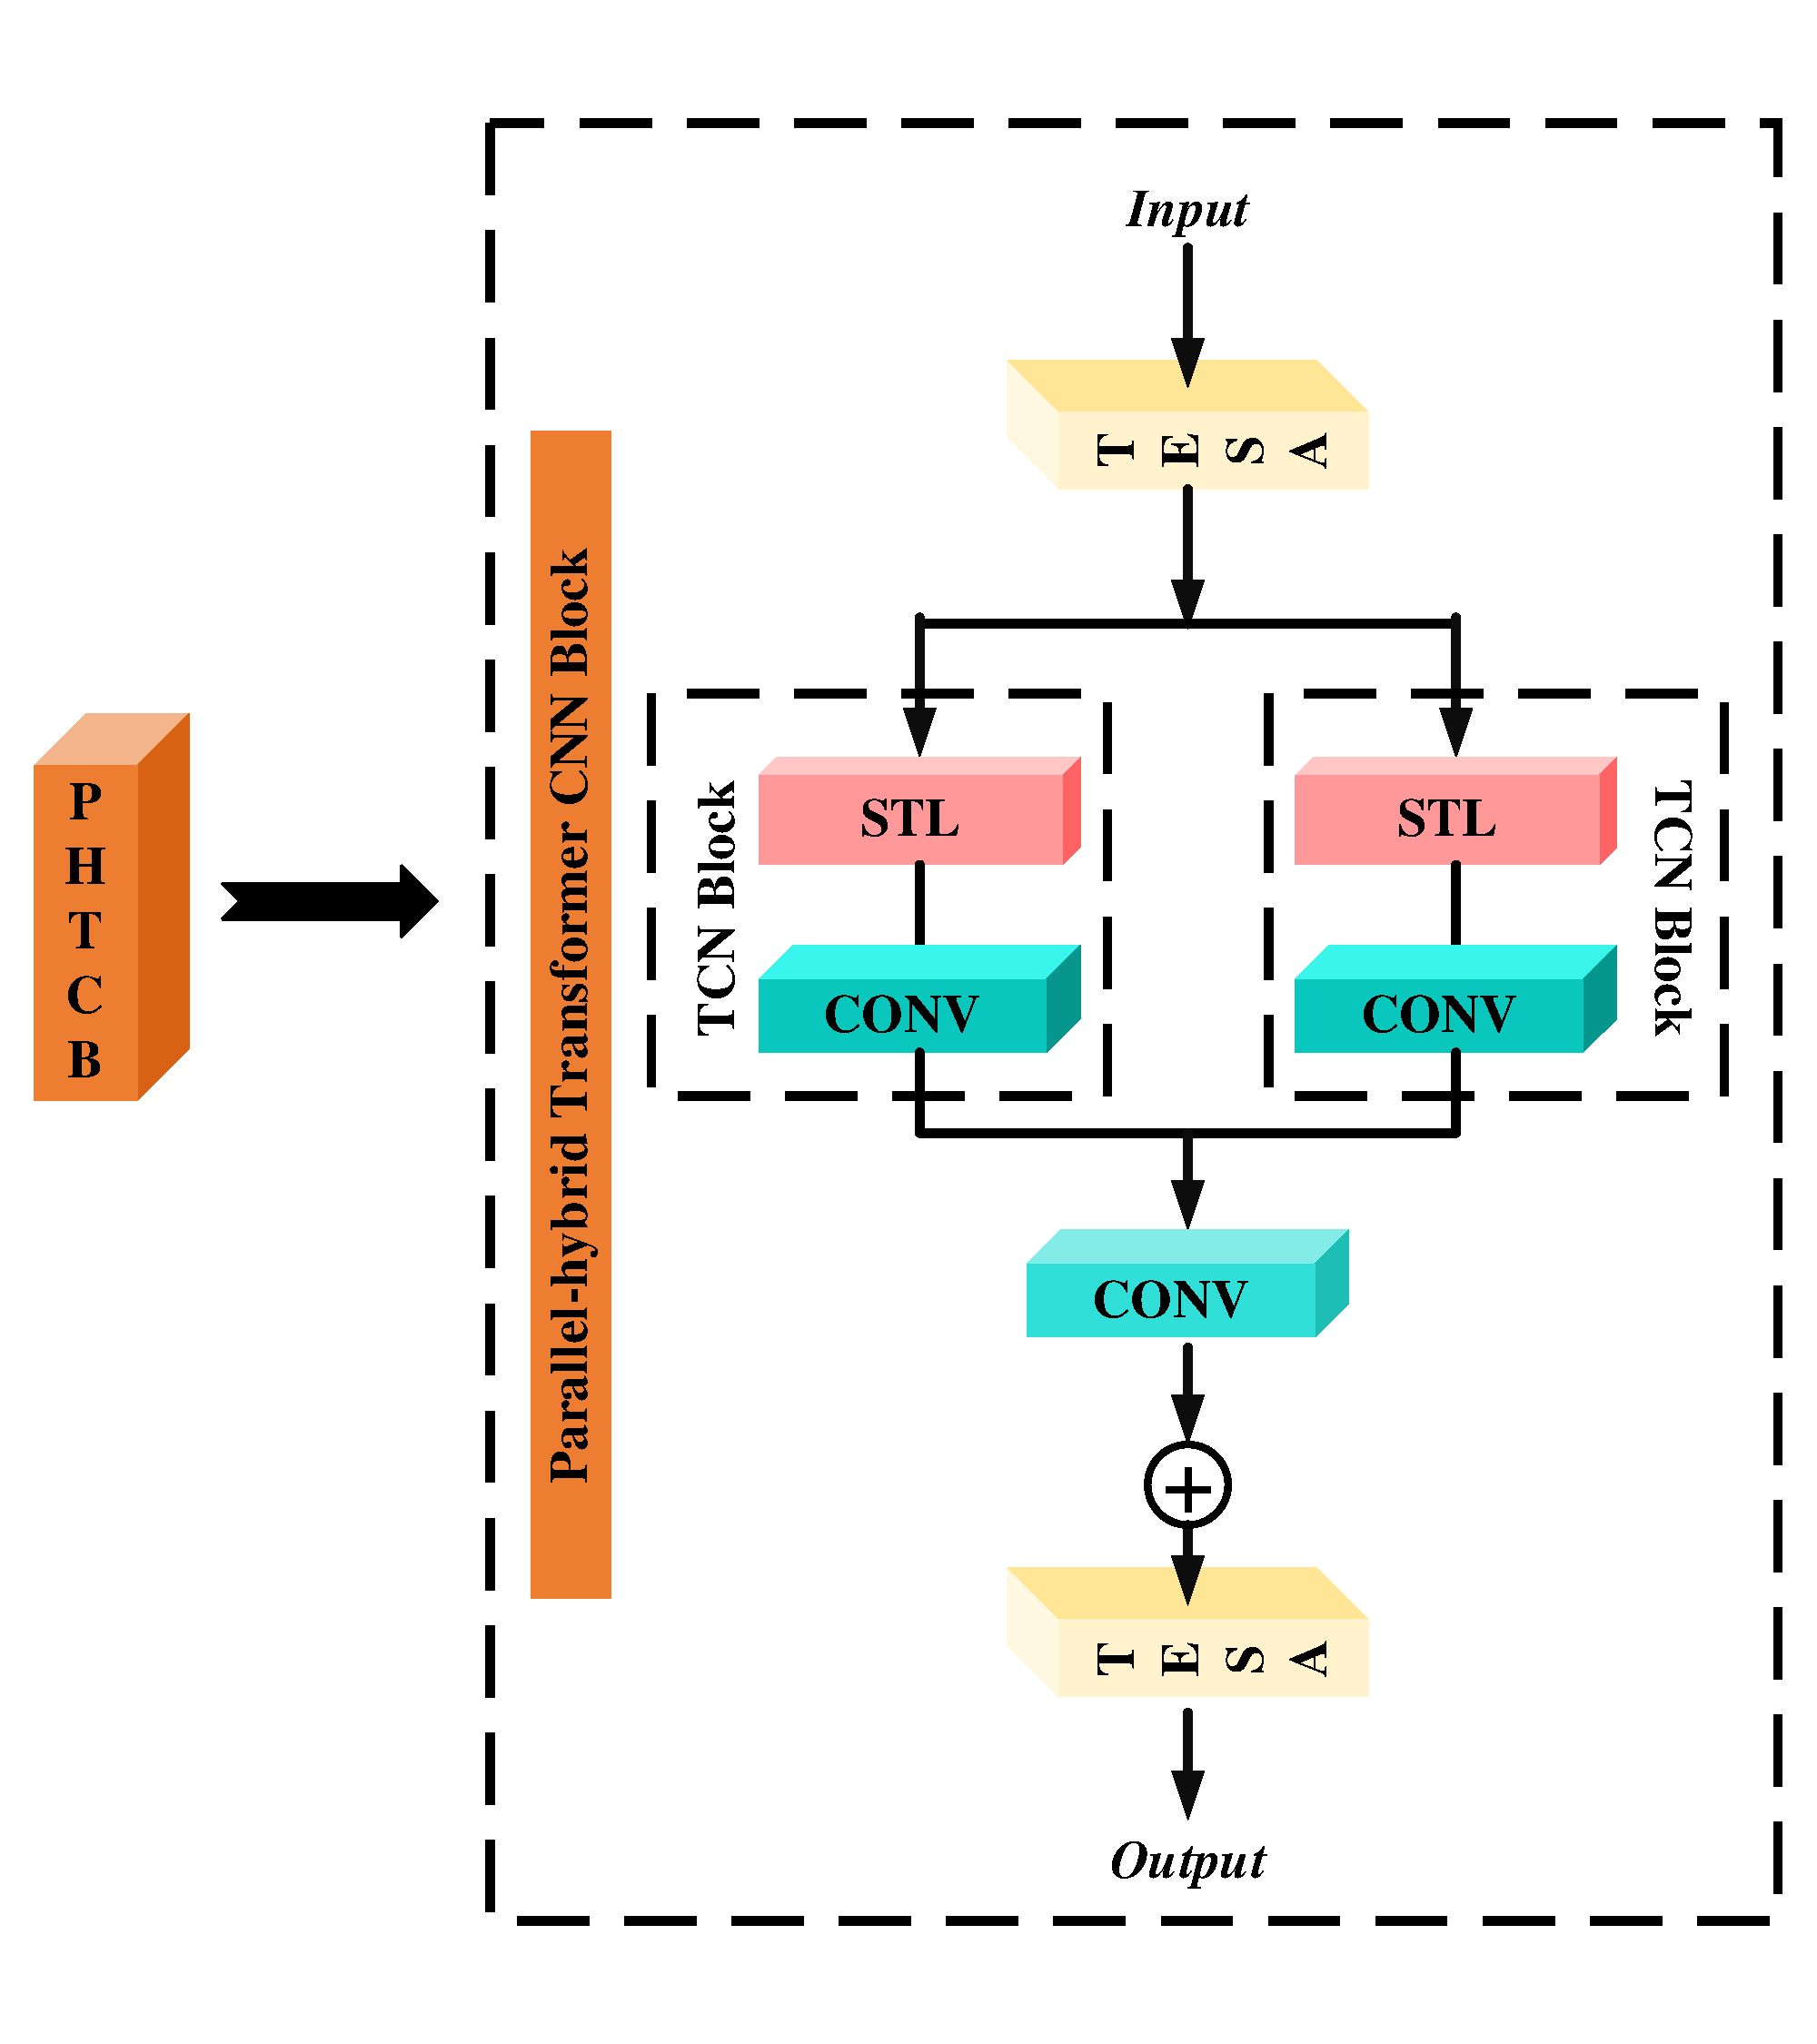
\includegraphics[width=\linewidth]{3FIGURE.pdf}
  \caption{The structure of Parallel Hybrid Transformer CNN Block (PHTCB).}
  \label{fig:3}
\end{figure}

\subsubsection{Transformer CNN (TCN) Block}

As already seen in Figure 2, the Transformer CNN (TCN) Block is the a hybrid block former by cascading the Swin transformer Layer and the CNN layer. It combines the powers of CNNS and Transformer to capture long range dependencies, reduce artifacts and simultaneously prevents the amplification of noise in super-resolution of noisy images. In our proposed architecture, we have used two TCN connected in paralled in each PHTCH. The output of the TCN Block is given in Equation 8. 

\begin{equation}
{H_{TCN}}= {F_{Conv3}}({F_{STL}}({H_{In}}),
\end{equation}

Here ${F_{STL}}$$(.)$ represents STL function, $({F_{Conv3}})$ is the 3 3 convolution operation, ${H_{In}}$ is the input of the TCN block and ${H_{TCN}}$ is the output of the TCN block.


\begin{figure}[ht]
  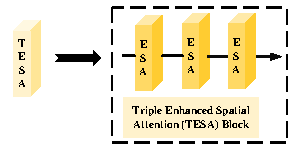
\includegraphics[width=\linewidth]{4FIGURE.pdf}
  \caption{The structure of Triple Enhanced Spatial Attention (TESA) Block.}
  \label{fig:4}
\end{figure}

\subsection{Enhanced spatial Attention (ESA)}

Enhanced Spatial Attention (ESA) is a critical components in image super-resolution (ISR) models, designed to selectively focus on significant features within an image. This mechanisms aims to improve the network’s ability to discern and enhance crucial details, such as edges, textures, and fine patterns, leading to higher-quality super-resolved images.

Enhanced Spatial Attention mechanisms refine traditional spatial attention by incorporating more sophisticated methods to identify and focus on critical image areas. This selective focus helps the network preserve and enhance fine details that are often lost in conventional methods. ESA dynamically adjusts the weights assigned to different regions based on the context and content of the image, allowing for adaptive attention that responds to varying image characteristics.

\begin{figure}[ht]
  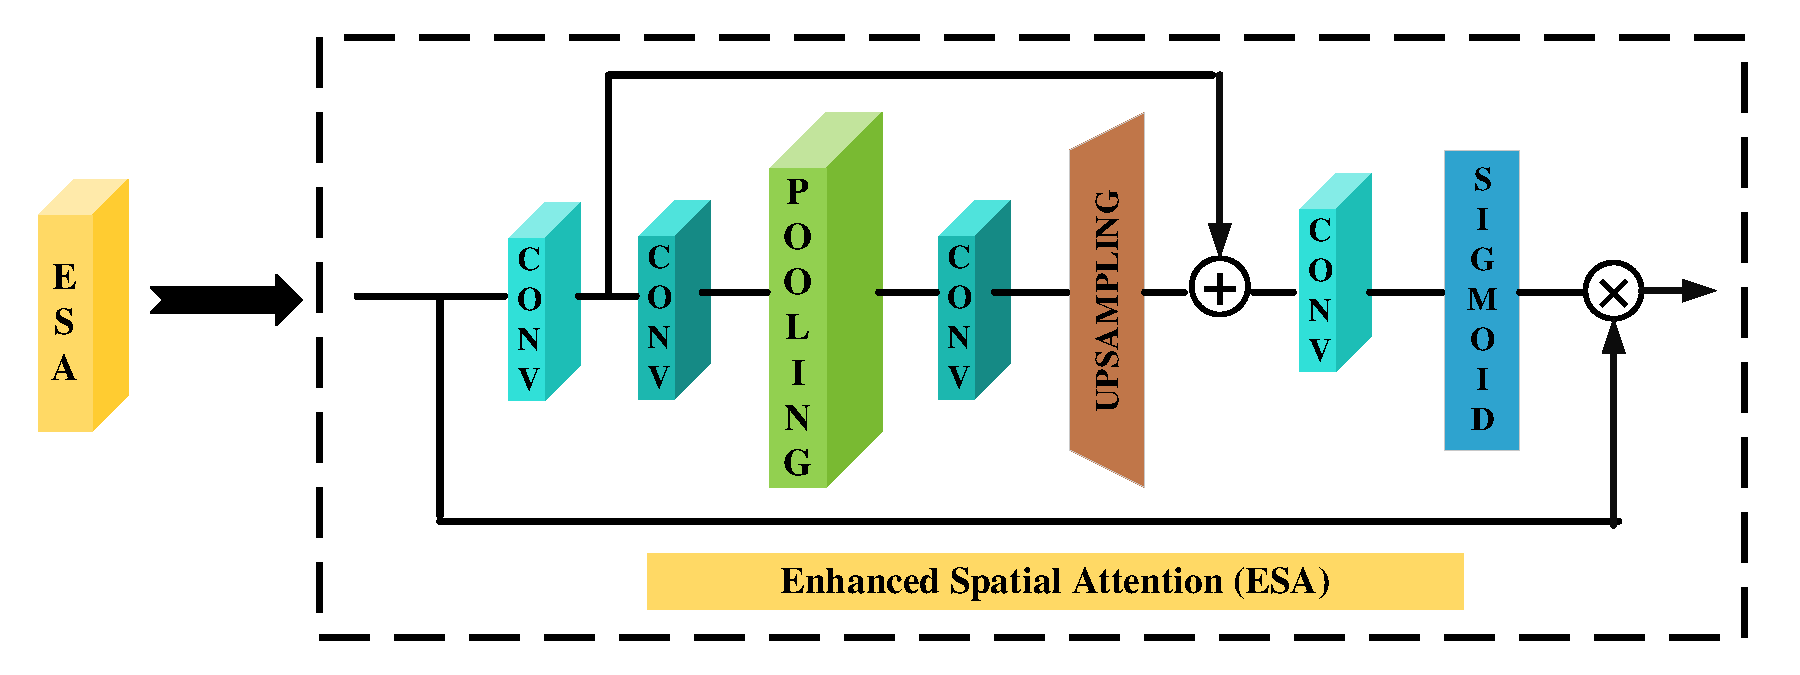
\includegraphics[width=\linewidth]{5FIGURE.pdf}
  \caption{Enhanced Spatial Attention (ESA).}
  \label{fig:4}
\end{figure}


Figure 5 shows diagram representation of the ESA mechanism, Attention maps are generated by adding the input feature maps through a series of convolutional, pooling and upsampling layers. These maps indicate the importance of each spatial location. The generated attention maps are then multiplied element-wise followed by an activation function (often sigmoid) with the input feature maps, emphasizing the significant regions while suppressing less important areas.

The mathematical expression of ESA is describes in Equations 9, 10, 11 and 12,

\begin{equation}
{H_{E1}}= {F_{up}}({F_{Conv3}}({F_{pool}}({F_{Conv3}}({F_{Conv1}}({H_{E1{i/p}}}))))),
\end{equation}

Here, ${H_{E1{i/p}}}$ is the input to the ESA, ${F_{Conv1}}$$(.)$ is the 1 $\times$ 1 convolution operation and ${F_{Conv3}}$$(.)$ is the 3 $\times$ 3 convolution operation fuction, ${F_{up}}$$(.)$ is the upsampling function and ${H_{E1}}$ is one of the input to the addition operation in ESA.
 
\begin{equation}
{H_{E2}}= {F_{Conv1}}({H_{E1{i/p}}}),
\end{equation}

${H_{E2}}$ is another input to the addition operation in ESA as seen in Figure 5.

\begin{equation}
{H_{E3}}= {H_{E1}} + {H_{E2}},,
\end{equation}

${H_{E3}}$ is the added output of the addition operation in ESA.

\begin{equation}
{H_{ESA}} = H_{E1} \times \sigma \left( F_{Conv3} \left( H_{E3} \right) \right)
\end{equation}

Here, $\times$ denotes the element wise multiplication, $\sigma$ denotes the sigmoid function and ${H_{ESA}}$ is the ouput of the Enhanced Spatial Attention (ESA) mechanism.


\subsection{Swin Transformer Layer (STL)}

The Swin Transformer layer is the transfomer component of the proposed architecture, which is designed for efficient and scalable vision tasks, including image super-resolution. Unlike the original STL which uses the components twice, we have used the components inside STL just once to reduce the computation  for self-attention across input feature map. It uses a hierarchical approach to model long-range dependencies and global context efficiently. We apply global self-attention across the entire input feature map. After each self-attention operation, a two-layer MLP is applied to transform the features further. Each MSA and MLP block is preceded by Layer Normalization to stabilize and improve the training process. Residual connections are used around each MSA and MLP block to enhance gradient flow and mitigate the vanishing gradient problem.

\begin{figure}[ht]
  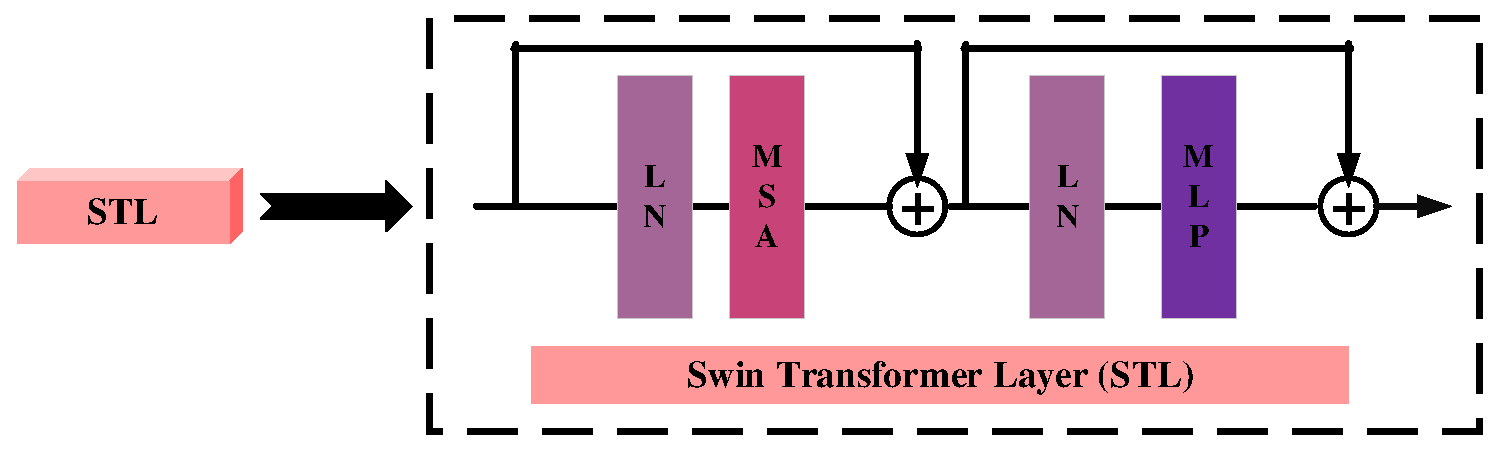
\includegraphics[width=\linewidth]{6FIGURE.pdf}
  \caption{ Inception Block }
  \label{fig:6}
\end{figure}

Figure 6 represents the STL used in our proposed method.  The mathematical expression for STL is given by Equations 13 and 14.

\begin{equation}
{H_{S1}}= {H_{S1{i/p}}} + ({F_{LN}}({F_{MSA}}({H_{S1{i/p}}}))),
\end{equation}

Here, ${H_{S1{i/p}}}$ is the input to the STL, ${F_{MSA}}$$(.)$ is the Multi-Head Self Attention function, ${F_{LN}}$$(.)$ is the Layer Normalization function, and ${H_{S1}}$ isthe output of the addition operation.

\begin{equation}
{H_{STL}}= {H_{S1}} + ({F_{LN}}({F_{MLP}}({H_{S1}}))),
\end{equation}

Here, ${F_{MLP}}$$(.)$ is Multi-Layer Perceptron, ${H_{STL}}$ is final output of the STL.


\section{Experimental Results}

In the experimental results section we have demonstrated the results of various qualitative, quantitative experiments conducted on our proposed method. We have also shown the comarative analyss of our proposed DHTCUN for parameters, average PSNR as well as SSIM, execution time and time complexiety of our proposed method. Furthermore ablation study has also been conducted by checking different number of PHTCB block to be used in model, bt changing the structure of TCN block and by changing the configuration of TCN block in PHTCH, PSNR versus Multi add analysis and finally convergence analysis of the model.

\subsection{Experimental Setup} 
In order to test the efficacy of our suggested model on publicly available datasets, this section presents the evaluation metrics, training specifics, and datasets. It should be mentioned that the testing and training sets are not the same. 

\subsubsection{Training and Testing Setup} 

Training our model involved randomly cropping low-resolution patches of 48 $\times$ 48. A window size of 24 $\times$ 24 has been selected.For $\times$2, $\times$3, $\times$4, and $\times$8, low-resolution images were created using MATLAB R2022b. To train the proposed network, a 24-GB NVIDIA GeForce GTX 2080ti GPU is utilized. Python 3.6 and the PyTorch 1.1.0 platform were used to write the algorithm for the proposed model. Model training involves obtaining  800 high-quality samples from DIV2K [41] datasets. We choose an Adam optimizer with $\beta_2 = 0.99$ and $\beta_1 = 0.90$ for optimization. For every 200 epochs, the learning rate of the suggested model is halved from 10$^{-4}$. 

Five common benchmark datasets, namely Set5 [42], Set14 [43], BSD100 [44], Urban100 [45], and Manga109 [46], were used to test our proposed model. Bicubic kernels are used to downsample the HR images in order to produce the LR image. Each batch size of eight training samples is divided up. Furthermore, by flipping and rotating at random angles of 90, 180, and 270 degrees, data augmentation produces extra samples for the computation. The image intensity range [-1, 1] has been used to compute the Mean Squared Error (MSE). Standard evaluation metrics like PSNR and SSIM can be used to quantitatively compare our model with the most advanced techniques.

\subsection{Quantitative evaluations in comparison to state-of-the-art methods}
Five benchmark test datasets are tabulatedly compared using standard metrics in Table 1. We quantitatively compare our proposed DHTCUN with seventeen SOTA methods: Bicubic, SRCNN [5], FSRCNN [6], VDSR [7], RDN [47], LapSRN [8], SENext [33], RCAN [11], MemNet [9], MFCC [32], EDSR [10], HAN [31], SwinIR [15], and NLSN [12], SRFormer [17], TCDFN [19], HNCT [20], MSRN [48], AWSRN [49], DBPN [50] and RDN [51]. 
Our suggested DHTCUN quantitative results have considerably surpassed the state-of-the-art techniques in terms of PSNR and SSIM, as indicated in Table 1. For scale factors $\times2$, $\times3$, $\times4$, and $\times8$, our suggested DHTCUN model performs better across all test datasets. Additionally, when compared to other SOTA models, our suggested approach produced a higher average PSNR/SSIM value on all image SR test datasets.


\begin{table*}
\caption{Comparison of the most sophisticated SR methods for upscaling factors $\times 2$, $\times 3$, $\times 4$, and $\times 8$ with our suggested DHTCUN evaluated using standard metrics. The highest score is displayed in bold and is colored {\color{red}\textbf{Red }}. {\color{blue}\underline{Blue}} indicates and displays the score that comes in second place.}

\label{table2}
\setlength{\tabcolsep}{4.5 pt}
\begin{tabular}{|c|c|c|cc|cc|cc|cc|cc|cc|}
\hline
\multirow{2}{*}{Method} & \multirow{2}{*}{Factor} & \multirow{2}{*}{\#Param}& \multicolumn{2}{c|}{Set5 [42]}& \multicolumn{2}{c|}{Set14 [43]}& \multicolumn{2}{c|}{BSD100 [44]}& \multicolumn{2}{c|}{Urban100 [45]}& \multicolumn{2}{c|}{Manga109 [46]}& \multicolumn{2}{c|}{Average}\\


 \cline{4-15}&&& \multicolumn{1}{c|}{PSNR$\uparrow$}  & SSIM{$\uparrow$}   & \multicolumn{1}{c|}{PSNR$\uparrow$}  & SSIM {$\uparrow$}   & \multicolumn{1}{c|}{PSNR$\uparrow$}  & SSIM {$\uparrow$}   & \multicolumn{1}{c|}{PSNR$\uparrow$}  & SSIM {$\uparrow$}  & \multicolumn{1}{c|}{PSNR$\uparrow$}  & SSIM {$\uparrow$}   & \multicolumn{1}{c|}{PSNR$\uparrow$}  & SSIM {$\uparrow$}  \\
 \hline

Bicubic&$\times2$ & -/-& \multicolumn{1}{c|}{33.68 } & 0.9304  & \multicolumn{1}{c|}{30.24 } &0.8691  & \multicolumn{1}{c|}{29.56 } & 0.8435  & \multicolumn{1}{c|}{26.88 } & 0.8405  & \multicolumn{1}{c|}{31.05 } & 0.9349&
\multicolumn{1}{c|}{30.23} & 0.8832 \\


SRCNN [5] & $\times 2$ & 57K& \multicolumn{1}{c|}{36.66 } & 0.9542  & \multicolumn{1}{c|}{32.45 } & 0.9067  &\multicolumn{1}{c|}{31.36 } & 0.8879  & \multicolumn{1}{c|}{29.51 } &0.8946 & \multicolumn{1}{c|}{35.72} &0.9680
&\multicolumn{1}{c|}{33.11} & 0.9219\\

FSRCNN [6]& $\times 2$& 12K & \multicolumn{1}{c|}{36.98} &0.9556& \multicolumn{1}{c|}{32.62} & 0.9087 &\multicolumn{1}{c|}{31.50} &0.8904& \multicolumn{1}{c|}{29.58} &0.9009& \multicolumn{1}{c|}{36.62} &0.9710
&\multicolumn{1}{c|}{33.56} & 0.9260\\

VDSR [7]& $\times 2$&665K& \multicolumn{1}{c|}{37.53} & 0.9587 & \multicolumn{1}{c|}{33.05} & 0.9127 &\multicolumn{1}{c|}{31.90} & 0.8960& \multicolumn{1}{c|}{30.77} & 0.9141 & \multicolumn{1}{c|}{37.16} & 0.9740
&\multicolumn{1}{c|}{33.24} & 0.9314\\

MemNet [9] & $\times 2$&677K& \multicolumn{1}{c|}{37.78} & 0.9597  & \multicolumn{1}{c|}{33.28} &0.9142  &\multicolumn{1}{c|}{32.08} & 0.8978 & \multicolumn{1}{c|}{31.31} &0.9195  & \multicolumn{1}{c|}{37.72} &0.9740
&\multicolumn{1}{c|}{34.43} &0.9330\\

LapSRN [8] & $\times 2$&812K& \multicolumn{1}{c|}{37.52} & 0.9591 & \multicolumn{1}{c|}{32.99} & 0.9124 &\multicolumn{1}{c|}{31.80} & 0.8949 & \multicolumn{1}{c|}{30.41} &  0.9101 & \multicolumn{1}{c|}{37.53} &  0.9740
&\multicolumn{1}{c|}{33.87} & 0.9302\\

SENext [33] & $\times 2$ &97K& \multicolumn{1}{c|}{38.04} & {0.9608} & \multicolumn{1}{c|}{\color{blue}\underline{34.24}} &{ 0.9181} & \multicolumn{1}{c|}{32.21} & {0.8997}& \multicolumn{1}{c|}{32.43} &{0.9287}& \multicolumn{1}{c|}{38.79} &{0.9774} &\multicolumn{1}{c|}{35.14} & {0.9369}\\


%RDN [73]& $\times 2$& 21,900K & \multicolumn{1}{c|}{38.24} &0.9614 & \multicolumn{1}{c|}{34.01} & 0.9212 &\multicolumn{1}{c|}{32.34} &0.9017& \multicolumn{1}{c|}{32.89} &0.9353& \multicolumn{1}{c|}{39.18} &0.9780
%&\multicolumn{1}{c|}{35.33} & 0.9395\\

RCAN [11]& $\times 2$&16,000K& \multicolumn{1}{c|}{38.27} & 0.9614 & \multicolumn{1}{c|}{34.12} & 0.9216 &\multicolumn{1}{c|}{32.41} & 0.9027& \multicolumn{1}{c|}{33.34} & 0.9384 & \multicolumn{1}{c|}{39.44} & 0.9786
&\multicolumn{1}{c|}{35.52} & 0.9405\\

%RNAN [75]& $\times 2$&1,350K& \multicolumn{1}{c|}{38.17} & 0.9611 & \multicolumn{1}{c|}{33.87} &0.9207 &\multicolumn{1}{c|}{32.32} & 0.9014& \multicolumn{1}{c|}{32.73} &0.9340 & \multicolumn{1}{c|}{39.23} & 0.9785
%&\multicolumn{1}{c|}{35.26} & 0.9391\\

MFCC [32]& $\times 2$&1,861K& \multicolumn{1}{c|}{38.16} & 0.9606 & \multicolumn{1}{c|}{33.85} &0.9195 &\multicolumn{1}{c|}{32.28} & 0.9010& \multicolumn{1}{c|}{32.65} &0.9331 & \multicolumn{1}{c|}{39.11} & 0.9780
&\multicolumn{1}{c|}{35.21} & 0.9384\\

%SRFBN [36]& $\times 2$&3,500K& \multicolumn{1}{c|}{38.11} &  0.9609  & \multicolumn{1}{c|}{33.82 } & 0.9196  &\multicolumn{1}{c|}{32.29} & 0.9010 & \multicolumn{1}{c|}{32.62} & 0.9328 & \multicolumn{1}{c|}{39.08} & 0.9779
%&\multicolumn{1}{c|}{35.18} &0.9384\\

%SAN [51]& $\times 2$&1,550K& \multicolumn{1}{c|}{38.31} &{\color{blue}\underline{0.9620}} & \multicolumn{1}{c|}{34.07} & 0.9213 &\multicolumn{1}{c|}{32.42} &0.9028& \multicolumn{1}{c|}{33.10} &0.9370 & \multicolumn{1}{c|}{39.32} & 0.9792
%&\multicolumn{1}{c|}{35.44} &0.9404\\

EDSR [10] & $\times 2$&43,000K& \multicolumn{1}{c|}{38.11} & 0.9602 & \multicolumn{1}{c|}{33.92} & 0.9195  &\multicolumn{1}{c|}{32.32} & 0.9013 & \multicolumn{1}{c|}{32.93} & 0.9351  & \multicolumn{1}{c|}{39.10} & 0.9773
&\multicolumn{1}{c|}{35.28} &0.9386\\

HAN [31] & $\times 2$&3,230K& \multicolumn{1}{c|}{38.27} & 0.9614  & \multicolumn{1}{c|}{34.16} & 0.9217  &\multicolumn{1}{c|}{32.41} & 0.9027 & \multicolumn{1}{c|}{33.35} &0.9385& \multicolumn{1}{c|}{39.46} & 0.9785
&\multicolumn{1}{c|}{35.53} &0.9405\\

NLSN [12] & $\times 2$ &4,475K& \multicolumn{1}{c|}{38.34} & 0.9618 & \multicolumn{1}{c|}{34.08} & 0.9231 & \multicolumn{1}{c|}{32.43} & 0.9027 & \multicolumn{1}{c|}{33.42} &0.9394 & \multicolumn{1}{c|}{39.59} & 0.9789
&\multicolumn{1}{c|}{35.57} & 0.9412\\

SwinIR [15] & $\times 2$ &878K& \multicolumn{1}{c|}{38.38} & {0.9620} & \multicolumn{1}{c|}{\color{blue}\underline{34.24}} &{ 0.9233} & \multicolumn{1}{c|}{32.47} & {0.9032} & \multicolumn{1}{c|}{33.51} & {\color{blue}\underline{0.9401}} & \multicolumn{1}{c|}{\color{red}\textbf{39.70}} &{\color{red}\textbf{0.9794}} &\multicolumn{1}{c|}{35.66} & {\color{blue}\underline{ 0.9416}}\\

ELAN [18] & $\times 2$ &621K& \multicolumn{1}{c|}{38.36} & 0.9620 & \multicolumn{1}{c|}{34.20} & 0.9228 & \multicolumn{1}{c|}{32.45} & 0.9030 & \multicolumn{1}{c|}{33.44} &0.9391 & \multicolumn{1}{c|}{39.62} & 0.9783
&\multicolumn{1}{c|}{35.61} & 0.9412\\

SRFormer [17] & $\times 2$ &853K& \multicolumn{1}{c|}{\color{blue}\underline{38.45}} & {\color{blue}\underline{0.9622}} & \multicolumn{1}{c|}{34.21} &{\color{red}\textbf{ 0.9236}} & \multicolumn{1}{c|}{\color{blue}\underline{32.51}} & {\color{blue}\underline{0.9038}} & \multicolumn{1}{c|}{\color{blue}\underline{33.86}} & {\color{red}\textbf{0.9426}} & \multicolumn{1}{c|}{\color{blue}\underline{39.69}} & {\color{blue}\underline{0.9786}} &\multicolumn{1}{c|}{\color{blue}\underline{35.74}} & {\color{red}\textbf{ 0.9422}}\\

TCDFN [19] & $\times 2$ &573K& \multicolumn{1}{c|}{38.16} & 0.9612 & \multicolumn{1}{c|}{33.89} & 0.9206 & \multicolumn{1}{c|}{32.26} & 0.9002 & \multicolumn{1}{c|}{32.79} &0.9341 & \multicolumn{1}{c|}{39.12} & 0.9780
&\multicolumn{1}{c|}{35.24} & 0.9388\\

HNCT [20] & $\times 2$ &356K& \multicolumn{1}{c|}{38.08} & 0.9608 & \multicolumn{1}{c|}{33.65} & 0.9182 & \multicolumn{1}{c|}{32.22} & 0.9001 & \multicolumn{1}{c|}{32.22} &0.9294 & \multicolumn{1}{c|}{38.87} & 0.9774
&\multicolumn{1}{c|}{35.01} & 0.9372\\

DHTCUN (Ours) & $\times 2$ &2,375K& \multicolumn{1}{c|}{\color{red}\textbf{38.48}} &{\color{red}\textbf{0.9624}} & \multicolumn{1}{c|}{\color{red}\textbf{34.25} } &{\color{blue}\underline{0.9234}} & \multicolumn{1}{c|}{\color{red}\textbf{32.54}} &{\color{red}\textbf{0.9040}}& \multicolumn{1}{c|}{\color{red}\textbf{33.88}} &{\color{red}\textbf{0.9426}}& \multicolumn{1}{c|}{\color{red}\textbf{39.70}} &{\color{blue}\underline{0.9786}} &\multicolumn{1}{c|}{\color{red}\textbf{35.77}} & {\color{red}\textbf{0.9422}}\\
\hline

Bicubic&$\times3$ &-/-& \multicolumn{1}{c|}{30.40} & 0.8686  & \multicolumn{1}{c|}{27.54} & 0.7741 & \multicolumn{1}{c|}{27.21} & 0.7389 & \multicolumn{1}{c|}{24.46} & 0.7349  & \multicolumn{1}{c|}{26.95} &0.8566
&\multicolumn{1}{c|}{27.31} & 0.7945\\

SRCNN [5] & $\times3$ & 57K&\multicolumn{1}{c|}{32.75} & 0.9090  & \multicolumn{1}{c|}{29.29} & 0.8215  &\multicolumn{1}{c|}{28.41} & 0.7863  & \multicolumn{1}{c|}{26.24} &0.7991 & \multicolumn{1}{c|}{30.48} &0.9117
&\multicolumn{1}{c|}{29.44} & 0.8455\\

FSRCNN [6]& $\times3$ &12K& \multicolumn{1}{c|}{33.16} &0.9140& \multicolumn{1}{c|}{29.42} & 0.8242 &\multicolumn{1}{c|}{28.52} & 0.7893& \multicolumn{1}{c|}{26.41} &0.8064& \multicolumn{1}{c|}{31.10} &0.9210
&\multicolumn{1}{c|}{29.70} & 0.8516\\

VDSR [7]& $\times3$ &665K& \multicolumn{1}{c|}{33.66} & 0.9213 & \multicolumn{1}{c|}{29.78} & 0.8318 &\multicolumn{1}{c|}{28.83} & 0.7976& \multicolumn{1}{c|}{27.14} & 0.8279 & \multicolumn{1}{c|}{32.01} & 0.9340
&\multicolumn{1}{c|}{30.28} & 0.8624\\

MemNet [9] & $\times3$ &677K& \multicolumn{1}{c|}{34.09} &0.9248  & \multicolumn{1}{c|}{30.00} &0.8350  &\multicolumn{1}{c|}{28.96} & 0.8001 & \multicolumn{1}{c|}{27.56} & 0.8376 & \multicolumn{1}{c|}{32.51} &0.9369
&\multicolumn{1}{c|}{ 30.62} &0.8669\\

LapSRN [8] &$\times3$ &812K& \multicolumn{1}{c|}{33.82} & 0.9227  & \multicolumn{1}{c|}{29.79} & 0.8320  &\multicolumn{1}{c|}{28.82} & 0.7973  & \multicolumn{1}{c|}{27.07} & 0.8271 & \multicolumn{1}{c|}{32.21} & 0.9350
&\multicolumn{1}{c|}{30.36} & 0.8631\\

SENext [33] & $\times3$ &54K& \multicolumn{1}{c|}{34.32} &{0.9255}& \multicolumn{1}{c|}{\color{red}\textbf{31.08}} & {0.8419} & \multicolumn{1}{c|}{29.11} &{0.8047}& \multicolumn{1}{c|}{28.60} &{0.8519}& \multicolumn{1}{c|}{33.63} &{0.9451} &\multicolumn{1}{c|}{31.35} &{0.8738} \\

%RDN [73]& $\times3$ &21,900K& \multicolumn{1}{c|}{34.71} &0.9296& \multicolumn{1}{c|}{30.57} & 0.8468 &\multicolumn{1}{c|}{29.26} & 0.8093& \multicolumn{1}{c|}{28.80} &0.8653& \multicolumn{1}{c|}{34.13} &0.9484
%&\multicolumn{1}{c|}{31.49} & 0.8798\\

RCAN [11]& $\times3$ &16,000K& \multicolumn{1}{c|}{34.74} & 0.9299 & \multicolumn{1}{c|}{30.65} & 0.8482 &\multicolumn{1}{c|}{29.32} & 0.8111& \multicolumn{1}{c|}{29.09} & 0.8702 & \multicolumn{1}{c|}{34.44} & 0.9499
&\multicolumn{1}{c|}{31.64} & 0.8818\\

%RNAN [75]& $\times3$ &1,350K& \multicolumn{1}{c|}{34.66} & 0.9290 & \multicolumn{1}{c|}{30.52} & 0.8462 &\multicolumn{1}{c|}{29.32} & 0.8090& \multicolumn{1}{c|}{28.75} & 0.8646 & \multicolumn{1}{c|}{34.25} & 0.9483
%&\multicolumn{1}{c|}{31.50} & 0.8794\\

MFCC [32]& $\times 3$&2,230K& \multicolumn{1}{c|}{34.67} & 0.9294 & \multicolumn{1}{c|}{30.51} &0.8456 &\multicolumn{1}{c|}{29.22} & 0.8080& \multicolumn{1}{c|}{28.64} & 0.8616 & \multicolumn{1}{c|}{34.15} & 0.9478
&\multicolumn{1}{c|}{31.43} & 0.8793\\

%SRFBN [36]&$\times3$ &3,500K& \multicolumn{1}{c|}{34.70} & 0.9292 & \multicolumn{1}{c|}{30.51} &0.8461 &\multicolumn{1}{c|}{29.24} & 0.8084& \multicolumn{1}{c|}{28.73} & 0.8641 & \multicolumn{1}{c|}{34.18} & 0.9481
%&\multicolumn{1}{c|}{31.47} & 0.8791\\

%SAN [51]& $\times3$ &1,550K& \multicolumn{1}{c|}{34.75} &  0.9300 & \multicolumn{1}{c|}{30.59} & 0.8476 &\multicolumn{1}{c|}{29.33} & 0.8112 & \multicolumn{1}{c|}{28.93} & 0.8671 & \multicolumn{1}{c|}{34.30} & 0.9494
%&\multicolumn{1}{c|}{31.58} &  0.8810\\

EDSR [10]& $\times3$&43,000K& \multicolumn{1}{c|}{34.65} & 0.9280 & \multicolumn{1}{c|}{30.52} & 0.8462 &\multicolumn{1}{c|}{29.25} & 0.8093& \multicolumn{1}{c|}{28.80} & 0.8653 & \multicolumn{1}{c|}{34.17} & 0.9476
&\multicolumn{1}{c|}{31.48} &0.8792\\

HAN [31] & $\times3$&3,230K& \multicolumn{1}{c|}{34.75} & 0.9299 & \multicolumn{1}{c|}{30.67} & 0.8483 &\multicolumn{1}{c|}{29.32} & 0.8110 & \multicolumn{1}{c|}{29.10} & 0.8705 & \multicolumn{1}{c|}{34.48} & 0.9500
&\multicolumn{1}{c|}{31.66} &0.8819\\

NLSN [12] & $\times3$ &4,475K& \multicolumn{1}{c|}{34.85} & 0.9306& \multicolumn{1}{c|}{30.70} &0.8485 &\multicolumn{1}{c|}{29.34} & 0.8117& \multicolumn{1}{c|}{29.25} & 0.8726& \multicolumn{1}{c|}{34.57} & 0.9508
&\multicolumn{1}{c|}{31.74} &0.8824\\

SwinIR [15] & $\times3$ &886K& \multicolumn{1}{c|}{34.89} & {0.9312} & \multicolumn{1}{c|}{30.77} &{0.8503} & \multicolumn{1}{c|}{29.37} & {0.8124} & \multicolumn{1}{c|}{29.29} & {0.8744}& \multicolumn{1}{c|}{34.74} &{0.9518} &\multicolumn{1}{c|}{31.81} & {0.8840}\\

ELAN [18] & $\times 3$ &629K& \multicolumn{1}{c|}{34.90} & 0.9313 & \multicolumn{1}{c|}{30.80} & 0.8504 & \multicolumn{1}{c|}{29.38} & 0.8124 & \multicolumn{1}{c|}{29.32} &0.8745 & \multicolumn{1}{c|}{34.73} & 0.9517
&\multicolumn{1}{c|}{31.82} & 0.8841\\

SRFormer [17] & $\times 3$ &861K& \multicolumn{1}{c|}{34.94} & {0.9318} & \multicolumn{1}{c|}{30.81} &{\color{red}\textbf{ 0.8518}} & \multicolumn{1}{c|}{29.41} & {\color{blue}\underline{0.8142}} & \multicolumn{1}{c|}{\color{red}\textbf{29.52}} & {\color{red}\textbf{0.8786}} & \multicolumn{1}{c|}{34.78} &{\color{blue}\underline{0.9524}} &\multicolumn{1}{c|}{\color{blue}\underline{31.89}} & {\color{red}\textbf{ 0.8857}}\\

TCDFN [19] & $\times 3$ &582K& \multicolumn{1}{c|}{34.63} & 0.8287 & \multicolumn{1}{c|}{30.56} & 0.8466 & \multicolumn{1}{c|}{29.23} & 0.8082 & \multicolumn{1}{c|}{28.71} &0.8624 & \multicolumn{1}{c|}{\color{red}\textbf{34.98}} & 0.9477
&\multicolumn{1}{c|}{31.62} & 0.8587\\

HNCT [20] & $\times 3$ &363K& \multicolumn{1}{c|}{\color{blue}\underline{34.96}} & {\color{red}\textbf{0.9329}} & \multicolumn{1}{c|}{30.88} & 0.8512 & \multicolumn{1}{c|}{\color{blue}\underline{29.42}} & 0.8132 & \multicolumn{1}{c|}{29.31} &0.8752 & \multicolumn{1}{c|}{34.88} & 0.9519
&\multicolumn{1}{c|}{\color{blue}\underline{31.89}} & 0.8848\\

DHTCUN (Ours) & $\times3$ &2,386K& \multicolumn{1}{c|}{\color{red}\textbf{34.98}} &{\color{blue}\underline{0.9320}}& \multicolumn{1}{c|}{\color{blue}\underline{30.89}} & {\color{blue}\underline{0.8515}}& \multicolumn{1}{c|}{\color{red}\textbf{29.44}} &{\color{red}\textbf{0.8143}}& \multicolumn{1}{c|}{\color{blue}\underline{29.34}} &{\color{blue}\underline{0.8754}}& \multicolumn{1}{c|}{\color{blue}\underline{34.91}} &{\color{red}\textbf{0.9526}} &\multicolumn{1}{c|}{\color{red}\textbf{31.91}} &{\color{blue}\underline{0.8852}}\\

\hline

Bicubic&$\times4$ &-/-& \multicolumn{1}{c|}{28.43 } &0.8109 & \multicolumn{1}{c|}{26.00  } &0.7023& \multicolumn{1}{c|}{25.96 } & 0.6678  & \multicolumn{1}{c|}{23.14 } & 0.6574  & \multicolumn{1}{c|}{25.15} &0.7890

&\multicolumn{1}{c|}{25.68} &0.7250\\


SRCNN [5] & $\times4$  &57K& \multicolumn{1}{c|}{30.48 } &0.8628   & \multicolumn{1}{c|}{27.50 } &0.7513  &\multicolumn{1}{c|}{ 26.90 } & 0.7103 & \multicolumn{1}{c|}{24.52 } &0.7226 & \multicolumn{1}{c|}{27.66 } &0.8580
&\multicolumn{1}{c|}{ 27.40} &0.7785 \\

FSRCNN [6]& $\times4$ &12K& \multicolumn{1}{c|}{30.70} & 0.8657& \multicolumn{1}{c|}{27.59} &0.7535  &\multicolumn{1}{c|}{26.96} &0.7128 & \multicolumn{1}{c|}{24.60} &0.7258 & \multicolumn{1}{c|}{27.89 } &0.8590
&\multicolumn{1}{c|}{27.57} &0.7850 \\

VDSR [7]& $\times4$ &665K & \multicolumn{1}{c|}{31.35} &0.8838 & \multicolumn{1}{c|}{28.02} & 0.7678&\multicolumn{1}{c|}{27.29} &0.7252 & \multicolumn{1}{c|}{25.18} &0.7525 & \multicolumn{1}{c|}{28.82 } & 0.8860
&\multicolumn{1}{c|}{28.13} &0.8031 \\

MemNet [9] & $\times4$ &677K& \multicolumn{1}{c|}{31.74} &0.8893& \multicolumn{1}{c|}{28.26} &0.7723 &\multicolumn{1}{c|}{27.40} &0.7281& \multicolumn{1}{c|}{25.50} &0.7630& \multicolumn{1}{c|}{29.42} & 0.8942
&\multicolumn{1}{c|}{28.46} &0.8094\\

LapSRN [8] & $\times4$ &812K& \multicolumn{1}{c|}{31.54} &0.8866 & \multicolumn{1}{c|}{28.09} &0.7694  &\multicolumn{1}{c|}{27.32} &0.7264  & \multicolumn{1}{c|}{25.21 } &0.7553   & \multicolumn{1}{c|}{29.09 } &0.8900
&\multicolumn{1}{c|}{28.27 } &0.8060 \\

SENext [33] & $\times4$  &54K& \multicolumn{1}{c|}{31.50} &0.8947  & \multicolumn{1}{c|}{28.99} &{0.7812}  & \multicolumn{1}{c|}{\color{red}\textbf{28.49}} &{0.7357} & \multicolumn{1}{c|}{26.64 } &{0.7839}  & \multicolumn{1}{c|}{30.48} &{0.9084}
&\multicolumn{1}{c|}{29.22} &{0.8208}    \\

%RDN [73]& $\times4$ &21,900K& \multicolumn{1}{c|}{32.47} & 0.8990& \multicolumn{1}{c|}{28.81} &0.7871  &\multicolumn{1}{c|}{27.72} &0.7419 & \multicolumn{1}{c|}{26.61} &0.8028 & %\multicolumn{1}{c|}{31.00 } &0.9151 &\multicolumn{1}{c|}{29.32} &0.8291 \\

RCAN [11]& $\times4$ &16,000K & \multicolumn{1}{c|}{32.63} &0.9002 & \multicolumn{1}{c|}{28.87} & 0.7889&\multicolumn{1}{c|}{27.77} &0.7436 & \multicolumn{1}{c|}{26.82} &0.8087 & \multicolumn{1}{c|}{31.22 } & 0.9173
&\multicolumn{1}{c|}{29.46} &0.8317 \\

%RNAN [75]& $\times4$ &1,350K& \multicolumn{1}{c|}{32.49} &0.8982  & \multicolumn{1}{c|}{28.83 } &0.7878 &\multicolumn{1}{c|}{27.72} &0.7421 & \multicolumn{1}{c|}{26.61 } &0.8023 & %\multicolumn{1}{c|}{31.09 } & 0.9149 &\multicolumn{1}{c|}{29.34 } &0.8291 \\

MFCC [32]& $\times 4$&2,157K& \multicolumn{1}{c|}{32.42} & 0.8973 & \multicolumn{1}{c|}{28.73} &0.7849 &\multicolumn{1}{c|}{27.67} & 0.7399 & \multicolumn{1}{c|}{26.48} &0.7977 & \multicolumn{1}{c|}{30.98} & 0.9131
&\multicolumn{1}{c|}{29.25} & 0.8265\\

%SRFBN [36]& $\times4$ &3,500K& \multicolumn{1}{c|}{32.47} &0.8983 & \multicolumn{1}{c|}{28.81} &0.7868 &\multicolumn{1}{c|}{27.72} &0.7409 & \multicolumn{1}{c|}{26.60} &0.8015 & \multicolumn{1}{c|}{31.15} & 0.9160
%&\multicolumn{1}{c|}{29.35} &0.8287  \\

%SAN [51]& $\times4$ &1,550K& \multicolumn{1}{c|}{32.64} &0.9003 & \multicolumn{1}{c|}{28.92} & 0.7888 &\multicolumn{1}{c|}{27.78} &0.7436 & \multicolumn{1}{c|}{26.79} &0.8068 & %%\multicolumn{1}{c|}{31.18} & 0.9169 &\multicolumn{1}{c|}{29.46} &0.8312 \\

EDSR [10] & $\times4$ &43,000K& \multicolumn{1}{c|}{32.46} &0.8968& \multicolumn{1}{c|}{28.80} &0.7876 &\multicolumn{1}{c|}{27.71} &0.7420 & \multicolumn{1}{c|}{26.64 } & 0.8033 & \multicolumn{1}{c|}{31.02} & 0.9148
&\multicolumn{1}{c|}{29.32} &0.8289  \\

HAN [31] & $\times4$ &3,230K& \multicolumn{1}{c|}{32.64 } &0.9002 & \multicolumn{1}{c|}{28.90} &0.7890 &\multicolumn{1}{c|}{27.80} &0.7442& \multicolumn{1}{c|}{26.85} &0.8094 & \multicolumn{1}{c|}{31.42} &0.9177
&\multicolumn{1}{c|}{29.52} &0.8321 \\

NLSN [12] & $\times4$ &4,475K& \multicolumn{1}{c|}{32.59 } &0.9000 & \multicolumn{1}{c|}{28.87} &0.7891 &\multicolumn{1}{c|}{27.78} &0.7444 & \multicolumn{1}{c|}{26.96} &0.8109 & \multicolumn{1}{c|}{31.27} &0.9184
&\multicolumn{1}{c|}{29.49} &0.8325 \\

SwinIR [15] & $\times4$  &897K& \multicolumn{1}{c|}{32.72} &{0.9021} & \multicolumn{1}{c|}{28.94} &{0.7914}& \multicolumn{1}{c|}{27.83} &{0.7459} & \multicolumn{1}{c|}{27.07} &{0.8164}& \multicolumn{1}{c|}{31.67} &{0.9226} &\multicolumn{1}{c|}{29.64} &{0.8356}  \\


ELAN [18] & $\times 4$ &621K& \multicolumn{1}{c|}{32.75} & 0.9022 & \multicolumn{1}{c|}{28.96} & 0.7914 & \multicolumn{1}{c|}{27.83} & 0.7459 & \multicolumn{1}{c|}{27.13} &0.8167 & \multicolumn{1}{c|}{31.68} & 0.9226 &\multicolumn{1}{c|}{29.67} & 0.8357\\

SRFormer [17] & $\times 4$ &873K& \multicolumn{1}{c|}{\color{blue}\underline{32.81}} & {\color{red}\textbf{0.9029}} & \multicolumn{1}{c|}{\color{red}\textbf{29.01}} &{ 0.7919} & \multicolumn{1}{c|}{27.85} & {\color{blue}\underline{0.7472}} & \multicolumn{1}{c|}{27.20} & {\color{blue}\underline{0.8189}} & \multicolumn{1}{c|}{\color{blue}\underline{31.75}} &{\color{red}\textbf{0.9237}} &\multicolumn{1}{c|}{29.72} & {\color{blue}\underline{ 0.8369}}\\

TCDFN [19] & $\times 4$ &591K& \multicolumn{1}{c|}{32.44} & 0.8976 & \multicolumn{1}{c|}{28.79} & 0.7861 & \multicolumn{1}{c|}{27.71} & 0.7381 & \multicolumn{1}{c|}{26.51} &0.7981 & \multicolumn{1}{c|}{30.90} & 0.9151 &\multicolumn{1}{c|}{29.27} & 0.8270\\

HNCT [20] & $\times 4$ &372K& \multicolumn{1}{c|}{32.78} & {\color{blue}\underline{0.9028}} & \multicolumn{1}{c|}{\color{blue}\underline{28.98}} & {\color{blue}\underline{0.7928}} & \multicolumn{1}{c|}{27.97} & 0.7468 & \multicolumn{1}{c|}{\color{blue}\underline{27.32}} &{\color{blue}\underline{0.8189}} & \multicolumn{1}{c|}{31.74} & 0.9228 &\multicolumn{1}{c|}{\color{blue}\underline{29.76}} & 0.8368\\

DHTCUN (Ours) & $\times4$  &2,395K& \multicolumn{1}{c|}{\color{red}\textbf{32.83}} &{\color{red}\textbf{0.9029}}  & \multicolumn{1}{c|}{\color{red}\textbf{29.01}} &{\color{red}\textbf{0.7929}}  & \multicolumn{1}{c|}{\color{blue}\underline{27.98}} &{\color{red}\textbf{0.7474}} & \multicolumn{1}{c|}{\color{red}\textbf{27.34 }} &{\color{red}\textbf{0.8191}}  & \multicolumn{1}{c|}{\color{red}\textbf{31.78}} &{\color{blue}\underline{0.9230}} &\multicolumn{1}{c|}{\color{red}\textbf{29.79}} &{\color{red}\textbf{0.8371}}    \\
\hline

Bicubic&$\times8$ &-/-& \multicolumn{1}{c|}{24.40} &0.6580& \multicolumn{1}{c|}{23.10} &0.5660 & \multicolumn{1}{c|}{23.67} &0.5480& \multicolumn{1}{c|}{20.74} &0.5160 & \multicolumn{1}{c|}{21.47} & 0.6500
&\multicolumn{1}{c|}{22.68} & 0.5876     \\

SRCNN [5] & $\times8$ &57K& \multicolumn{1}{c|}{25.33} & 0.6900 & \multicolumn{1}{c|}{23.76} &0.5910 &\multicolumn{1}{c|}{24.13} &0.5660 & \multicolumn{1}{c|}{21.29} &0.5440& \multicolumn{1}{c|}{22.46} &0.6950
&\multicolumn{1}{c|}{23.42} & 0.5739      \\

FSRCNN [6]& $\times8$&12K& \multicolumn{1}{c|}{25.60} &0.6970 & \multicolumn{1}{c|}{24.00} &0.5990&\multicolumn{1}{c|}{24.31} &0.5720 & \multicolumn{1}{c|}{21.45} &0.5500 & \multicolumn{1}{c|}{22.72} & 0.6920
&\multicolumn{1}{c|}{23.46} &  0.5696      \\

VDSR [7]& $\times8$&665K& \multicolumn{1}{c|}{25.93} &0.7240& \multicolumn{1}{c|}{24.26} &0.6140 &\multicolumn{1}{c|}{24.49} &0.5830 & \multicolumn{1}{c|}{21.70} &0.5710 & \multicolumn{1}{c|}{23.16} &0.7250
&\multicolumn{1}{c|}{23.50} & 0.5800       \\

MemNet [9]& $\times8$&677K& \multicolumn{1}{c|}{26.16} &  0.7414 & \multicolumn{1}{c|}{24.38} & 0.6199&\multicolumn{1}{c|}{24.58} & 0.5842 & \multicolumn{1}{c|}{21.89  } &0.5825 & \multicolumn{1}{c|}{23.56 } &0.7387
&\multicolumn{1}{c|}{24.11  } &  0.6529       \\

LapSRN [8]& $\times8$&812K& \multicolumn{1}{c|}{26.15} &0.7380& \multicolumn{1}{c|}{24.35} &0.6200 &\multicolumn{1}{c|}{24.54} &0.5860 & \multicolumn{1}{c|}{21.81} &0.5810 & \multicolumn{1}{c|}{23.39} &0.7350
&\multicolumn{1}{c|}{24.04} & 0.6520       \\

MSRN [48]& $\times8$&6,226K& \multicolumn{1}{c|}{26.59} &  0.7254 & \multicolumn{1}{c|}{24.88} & 0.5961&\multicolumn{1}{c|}{24.70} & 0.5610 & \multicolumn{1}{c|}{22.37 } & 0.6077 & \multicolumn{1}{c|}{24.30 } &0.7701 &\multicolumn{1}{c|}{24.56  } &  0.6520       \\

EDSR [10]& $\times8$&43,000K& \multicolumn{1}{c|}{26.96} &  0.7762 & \multicolumn{1}{c|}{24.91} & 0.6420&\multicolumn{1}{c|}{24.81} & 0.5985 & \multicolumn{1}{c|}{22.51  } &0.6221 & \multicolumn{1}{c|}{24.69 } &0.7841
&\multicolumn{1}{c|}{24.74  } &  0.6824       \\

AWSRN [49]& $\times8$&2,348K& \multicolumn{1}{c|}{26.97} &  0.7747 & \multicolumn{1}{c|}{24.96} & 0.6414&\multicolumn{1}{c|}{24.80} & 0.5967 & \multicolumn{1}{c|}{22.45  } &0.6174 & \multicolumn{1}{c|}{24.69 } &0.7842 &\multicolumn{1}{c|}{24.77  } &  0.6828       \\

DBPN [50]& $\times8$&10,000K& \multicolumn{1}{c|}{26.96} &  0.7762 & \multicolumn{1}{c|}{24.91} & 0.6420&\multicolumn{1}{c|}{24.81} & 0.5985 & \multicolumn{1}{c|}{22.51  } &0.6221 & \multicolumn{1}{c|}{24.60 } &0.7732
&\multicolumn{1}{c|}{24.75  } &  0.6824       \\

MFCC [32]& $\times8$&2,453K& \multicolumn{1}{c|}{27.07} &  0.7762 & \multicolumn{1}{c|}{25.01} & 0.6412&\multicolumn{1}{c|}{24.84} & 0.5980 & \multicolumn{1}{c|}{22.54  } &0.6196 & \multicolumn{1}{c|}{24.63 } &0.7791 &\multicolumn{1}{c|}{24.81  } &  0.6828       \\

RDN [51]& $\times8$&21,900K& \multicolumn{1}{c|}{27.21} &  0.7840 & \multicolumn{1}{c|}{25.13} & 0.6480&\multicolumn{1}{c|}{24.88} & 0.6010 & \multicolumn{1}{c|}{22.73  } &0.6312 & \multicolumn{1}{c|}{25.14 } &0.7897 &\multicolumn{1}{c|}{25.02  } &  0.6907       \\

RCAN [11]& $\times8$&16,000K& \multicolumn{1}{c|}{27.31} &  0.7878 & \multicolumn{1}{c|}{25.23} & {\color{blue}\underline{0.6511}}&\multicolumn{1}{c|}{24.98} & 0.6058 & \multicolumn{1}{c|}{\color{blue}\underline{23.00}} &{\color{blue}\underline{0.6452}} & \multicolumn{1}{c|}{\color{blue}\underline{25.24 }} &{\color{blue}\underline{0.8029}}
&\multicolumn{1}{c|}{\color{blue}\underline{25.15}} &  {\color{blue}\underline{0.6985}}       \\

SENext [33] & $\times8$ &97K& \multicolumn{1}{c|}{26.87} &{0.7415} & \multicolumn{1}{c|}{\color{red}\textbf{25.73}} &{0.6200} & \multicolumn{1}{c|}{\color{red}\textbf{26.79}} &{0.5847} & \multicolumn{1}{c|}{21.90} &{0.5829} & \multicolumn{1}{c|}{23.96} &{0.7389} &\multicolumn{1}{c|}{25.05} &{0.6536}  \\


HAN [31] & $\times8$&3,230K& \multicolumn{1}{c|}{\color{blue}\underline{27.33}} &{\color{blue}\underline{0.7884}}   & \multicolumn{1}{c|}{25.24} & 0.6510   &\multicolumn{1}{c|}{24.98} &{\color{blue}\underline{0.6059}}   & \multicolumn{1}{c|}{22.98} &{0.6437} & \multicolumn{1}{c|}{25.20}  &{0.8011} &\multicolumn{1}{c|}{25.14} &{0.6980} \\


DHTCUN (Ours) & $\times8$ &2,405K& \multicolumn{1}{c|}{\color{red}\textbf{27.40}} &{\color{red}\textbf{0.7888}} & \multicolumn{1}{c|}{\color{blue}\underline{25.29}} &{\color{red}\textbf{0.6517}} & \multicolumn{1}{c|}{\color{blue}\underline{25.08}} &{\color{red}\textbf{0.6064}} & \multicolumn{1}{c|}{\color{red}\textbf{23.08}} &{\color{red}\textbf{0.6458}} & \multicolumn{1}{c|}{\color{red}\textbf{25.28}} &{\color{red}\textbf{0.8033}} &\multicolumn{1}{c|}{\color{red}\textbf{25.22}} &{\color{red}\textbf{0.6992}}  \\

\hline


\end{tabular}
\end{table*}



\subsection{Comparative study using the quantity of model parameters}
The parameters and PSNR comparison for our suggested DHTCUN model is displayed in Figure 7. The effectiveness of our suggested model, DHTCUN, with an scale factor of $\times 2$, is assessed using the Set5 [42] test dataset. Lowering the number of parameters indicates lower computational costs. The DHTCUN model more effectively reduces the model's size when compared to other state-of-the-art deep learning models. Around 92\% less parameters are found in DHTCUN than in EDSR [10], 81\% less in RCAN [11], 85\% less in RDN [51], 42\% less in NLSN [12], and 22\% less in HAN [31]. Comparing our suggested method to five other cutting-edge approaches, Figure 7 demonstrates that our suggested method has fewer parameters. This indicates our model's efficiency in reducing the compuattional burden.

\begin{figure}[ht]
  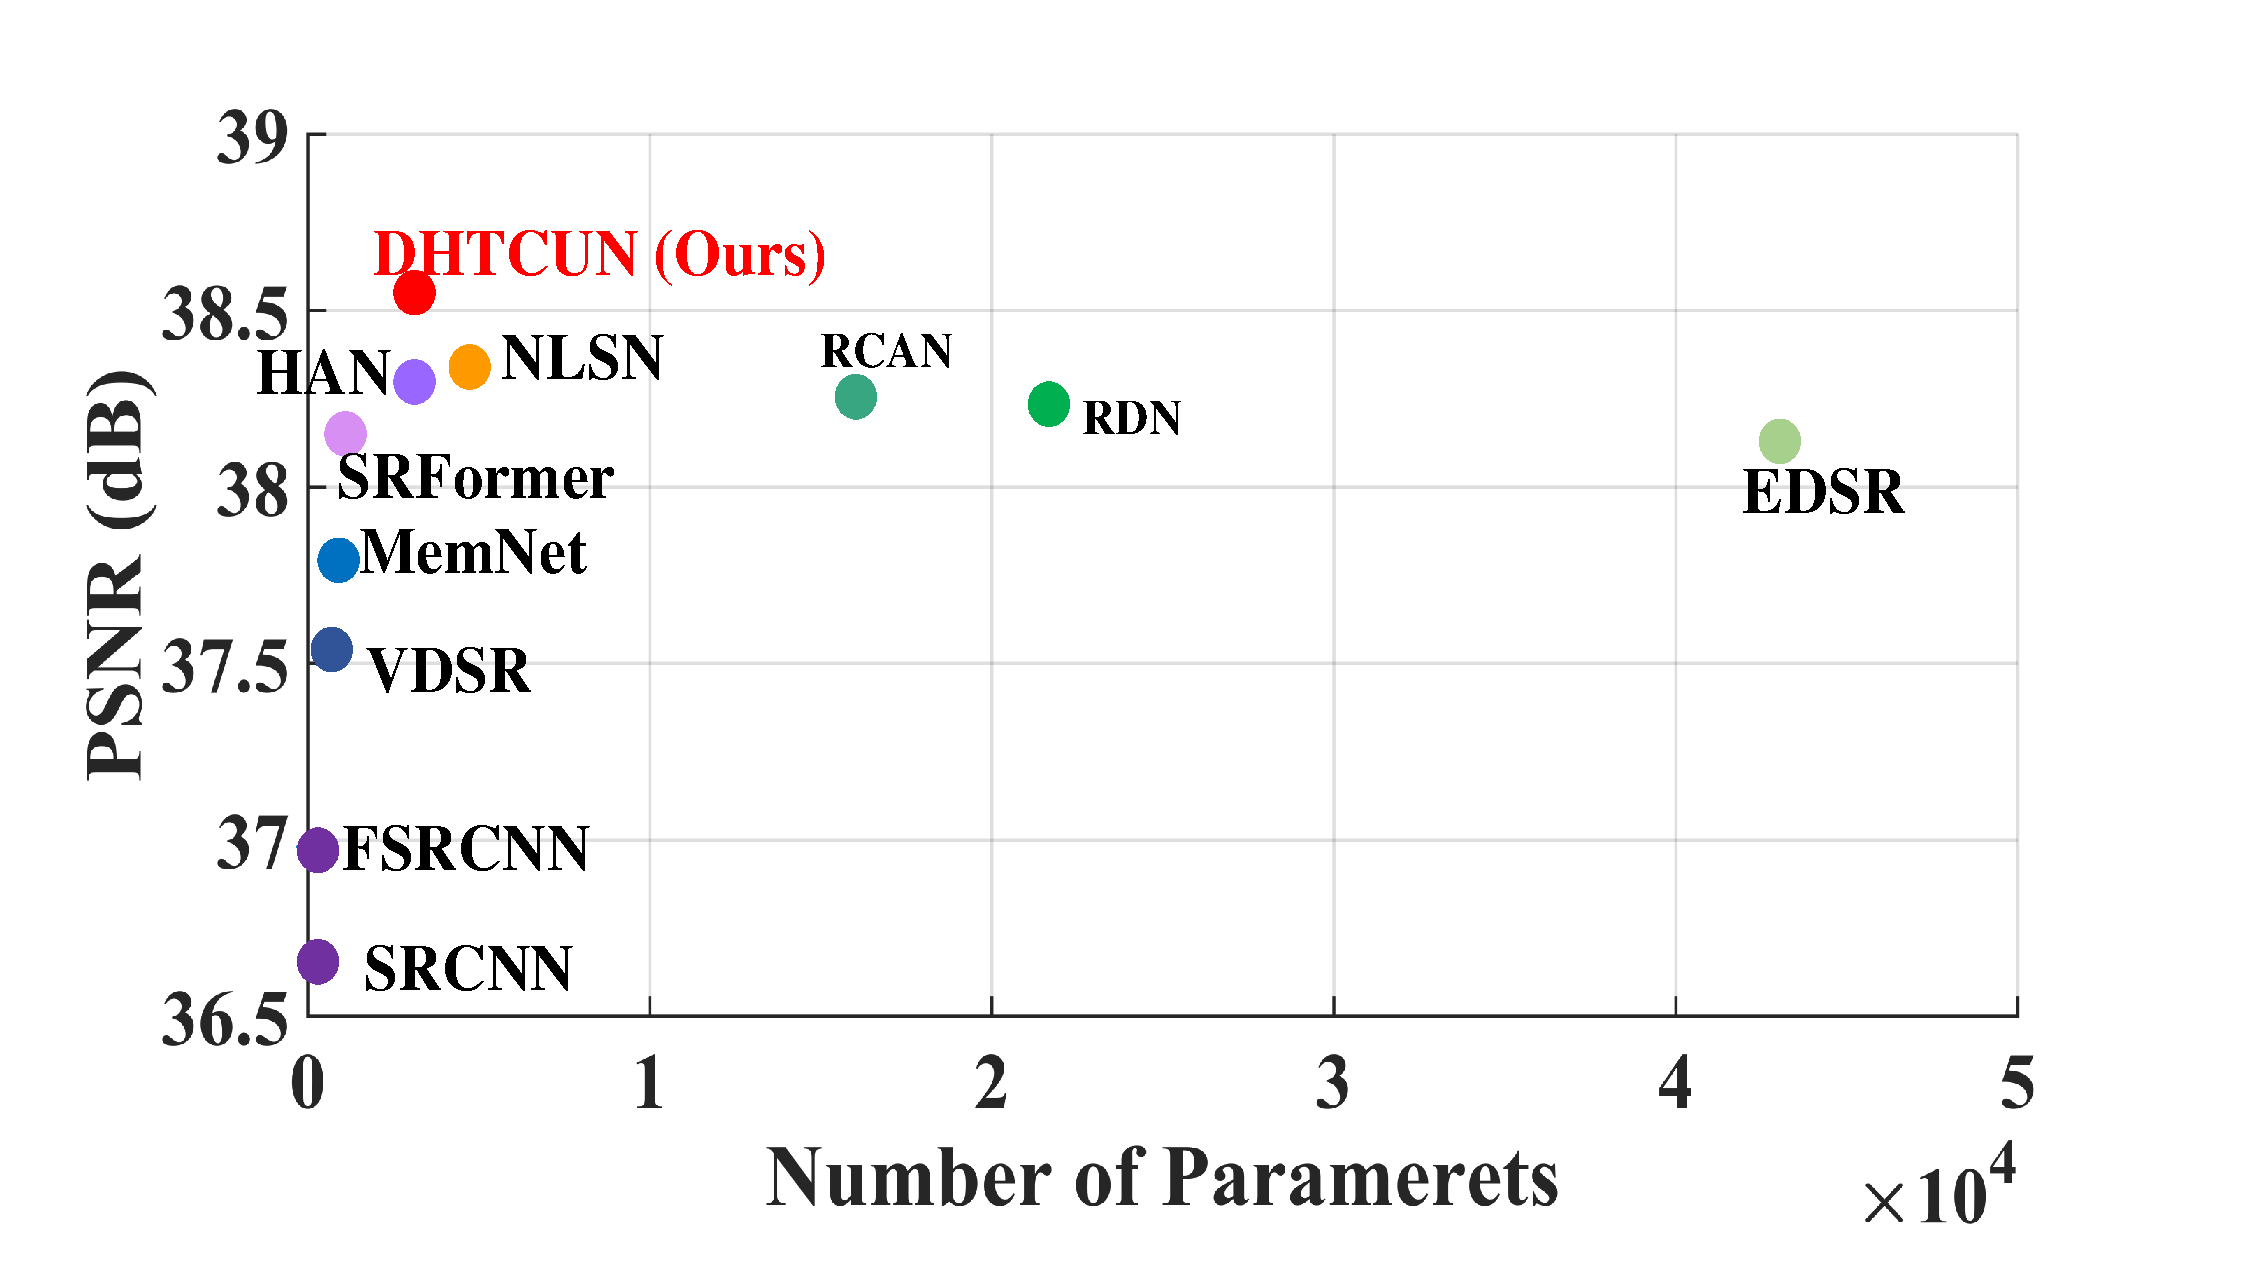
\includegraphics[width=\linewidth]{7FIGURE.pdf}
  \caption{Analysis of model parameters in relation to PSNR using the $\times2$ enlargement factor on the Set5 [42] image dataset.}
  \label{fig:7}
\end{figure}

\subsection{Comparison of the mean PSNR and SSIM of the Image SR Datasets for $\times$4 and $\times$8 enlargement factors. }

Using standard objective measures, Figures 8 and 9 compare the average PSNR and SSIM of various existing image SR methods on benchmark datasets (Set5 [42], Set14 [43], BSD100 [44], Urban100 [45], Manga109 [46]) for enlargement factors of $\times4$ and $\times8$. According to the quantitative results, our proposed DHTCUN outperforms HNCT [20], SRFormer [17], NLSN [12], RCAN[11], EDSR [10], and MemNet [9] when it comes to the enlargement factor of $\times4$, and SRCNN [5], LapSRN [8], MemNet [9], RCAN [11], HAN [31], RDN [51], EDSR [10], and AWSRN [49] when it comes to the enlargement factor of $\times8$. The average quantitative PSNR and SSIM values for Figure 8 and Figure 9 are given in Table 1.

\begin{figure}[ht]
  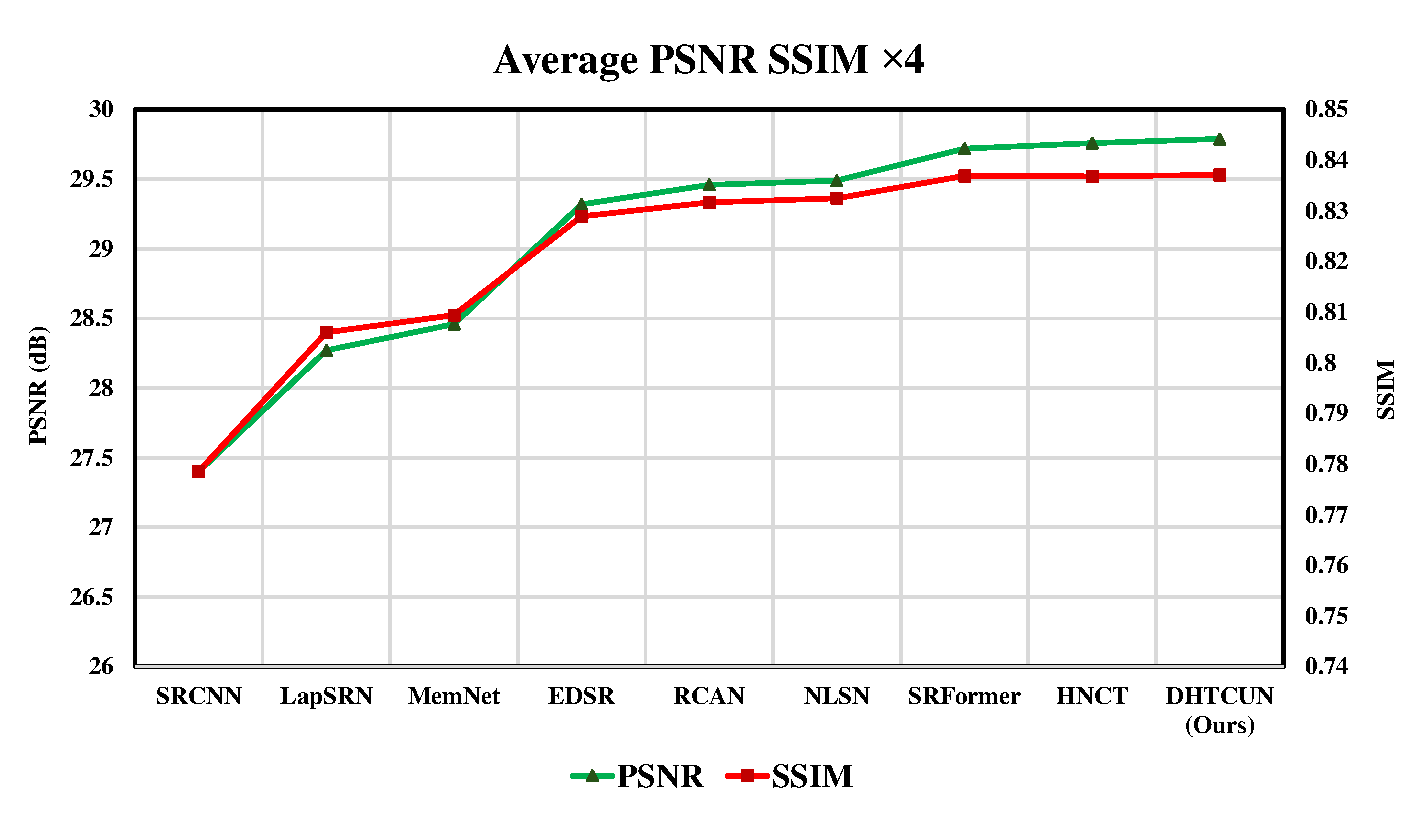
\includegraphics[width=\linewidth]{8FIGURE.pdf}
  \caption{Comparison of Image SR Test Data Sets for PSNR and SSIM based on $\times4$ enlargement factor.}
  \label{fig:8}
\end{figure}

\begin{figure}[ht]
  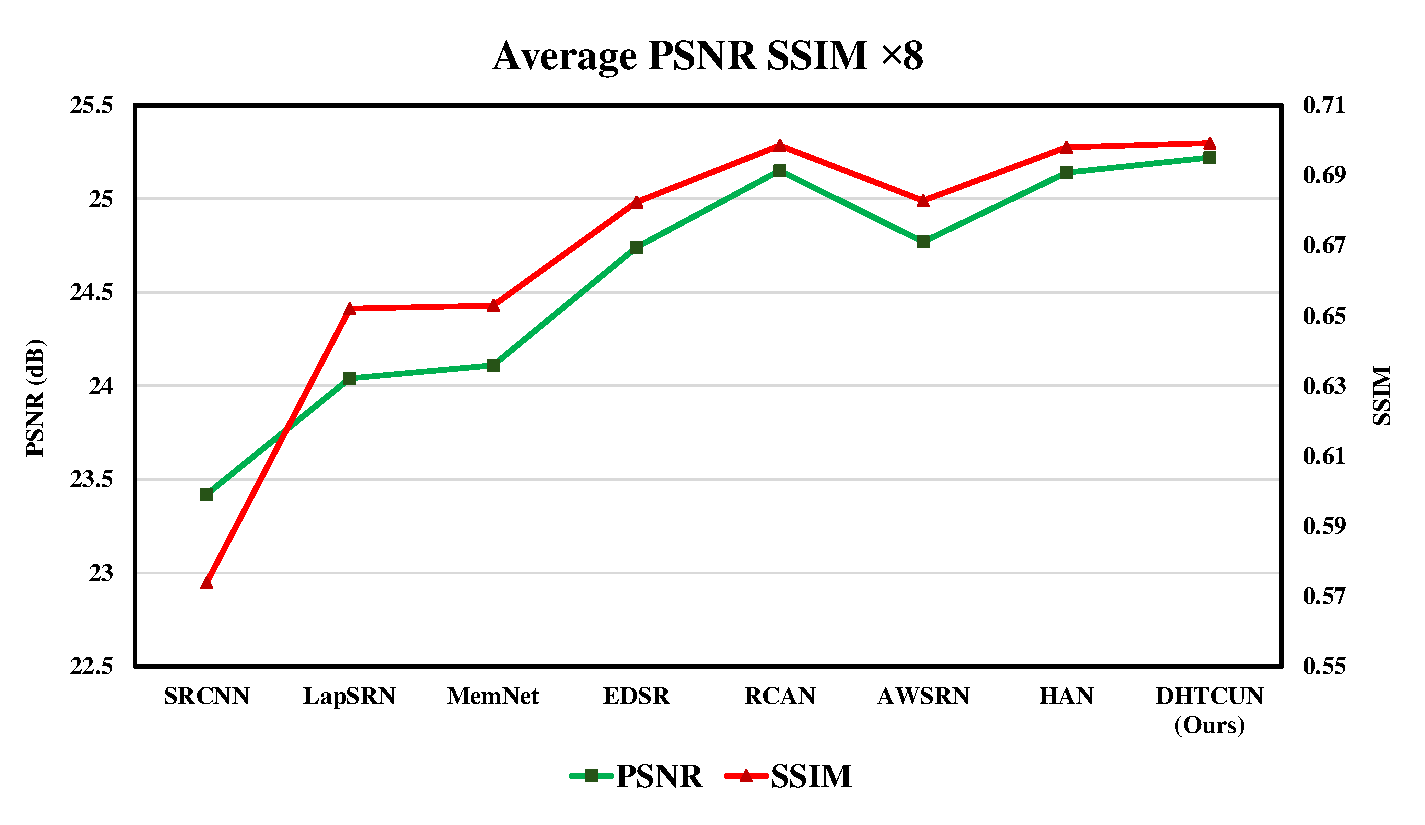
\includegraphics[width=\linewidth]{9FIGURE.pdf}
  \caption{Comparison of Image SR Test Data Sets for PSNR and SSIM based on an enlargement factor of $\times8$.}
  \label{fig:9}
\end{figure}

\subsection{PSNR versus execution time: A quantitative analysis }

Execution time refers to the duration required for an ISR model to process an image and produce a high-resolution output. As seen in Figure 10, this section displays the DHTCUN's performance in terms of PSNR versus execution time. The state-of-the-art techniques were assessed using an NVIDIA GeForce GTX 2080ti GPU with 24GB of memory. On Set14 [43] scale factor $\times4$, Figure 10 illustrates the trade-off between PSNR and execution time. Our suggested approach outperforms five state-of-the-art techniques (HNCT [20], SRFormer [17], NLSN [12], RNAN [52], and RDN [51]) with the highest PSNR of 29.06. 

\begin{figure}[ht]
  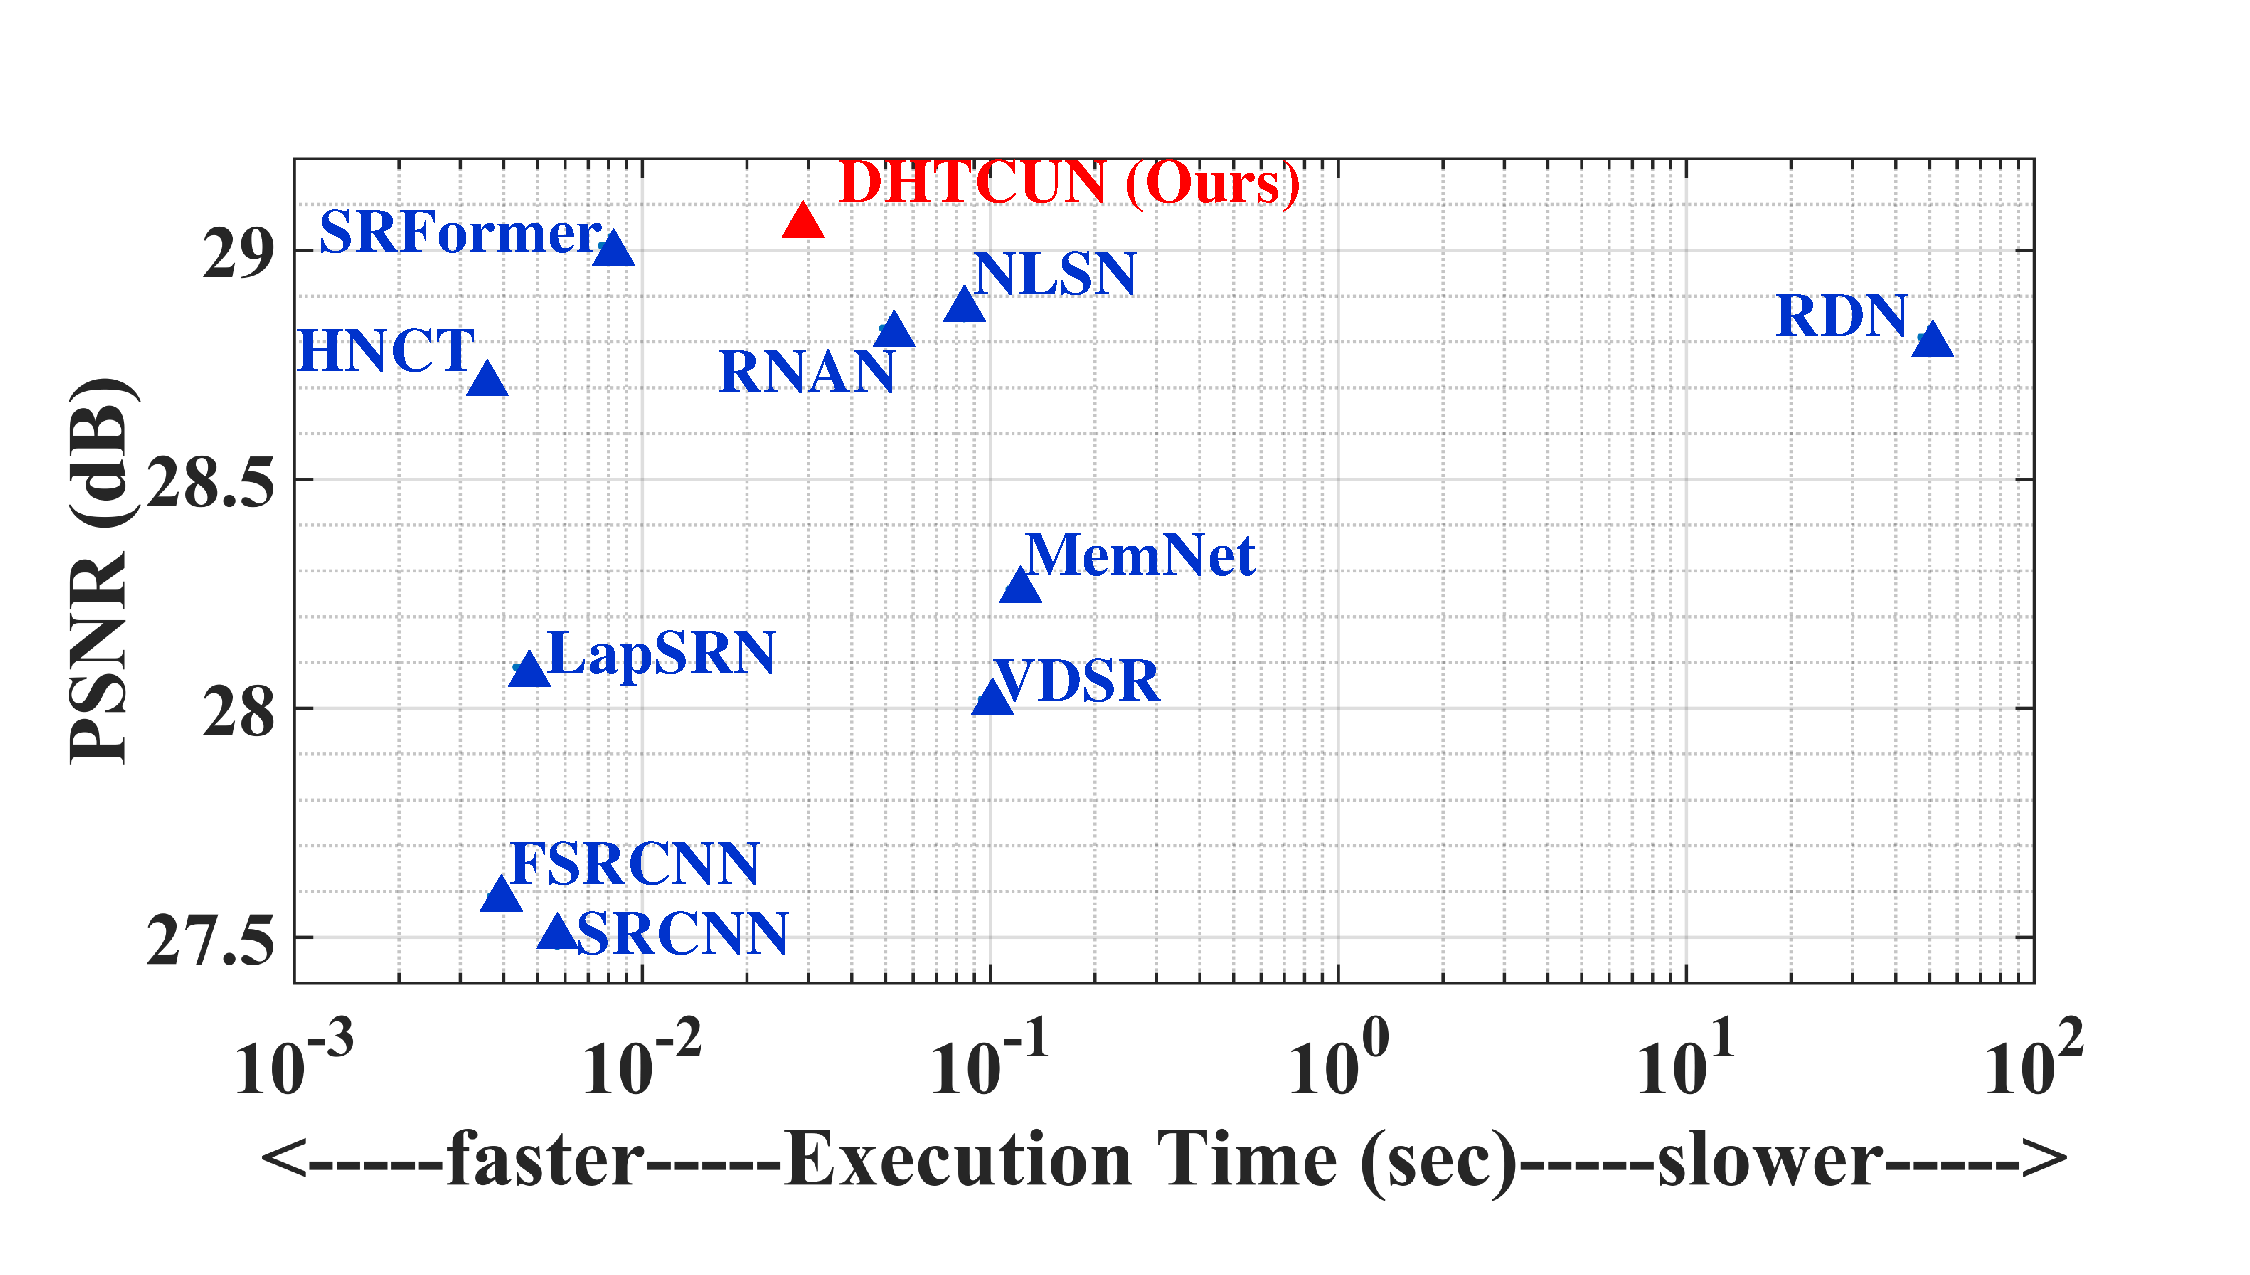
\includegraphics[width=\linewidth]{10FIGURE.pdf}
  \caption{Measurement of execution time against PSNR using a scale factor of $\times4$ on Set 14 [43].}
  \label{fig:10}
\end{figure}

\subsection{Examination of Time Complexity}

The length of time needed to finish each training epoch for a deep learning model illustrates how complex the model is in terms of time. The time complexity of these algorithms is a crucial factor, especially when aiming for real-time applications. The time complexity of image super-resolution (ISR) is primarily influenced by the size of the input image (\textit{n} × \textit{m}), the depth of the network \textit{d}, and the size of the convolutional kernel \textit{k}. 

The time required per epoch in 100 training epochs of the five state-of-the-art methods TCDFN [19], ELAN [18], HNCT [20], NLSN [12] and our suggested DHTCUN is displayed in Figure 11. There is a noticeable difference in the curves, suggesting that our suggested DHTCUN requires less training time for every epoch. DHTCUN therefore exhibits lower time complexity compared to the five state-of-the-art methods.

\begin{figure}[ht]
  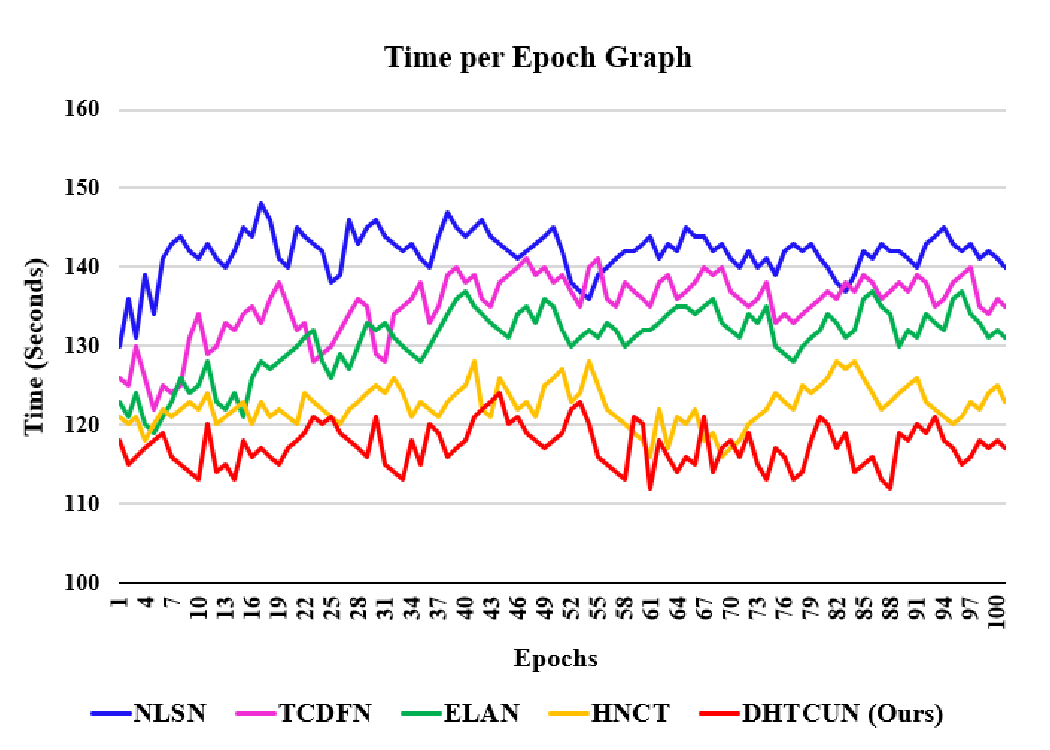
\includegraphics[width=\linewidth]{11FIGURE.pdf}
  \caption{Estimation of Time complexity on DIV2K [41] Dataset for 100 epochs on scale factor $\times$4.}
  \label{fig:11}
\end{figure}

\subsection{A Comparison of Visual Quality}
For image SR test datasets, including Set5 [42], Set14 [43], BSD100 [44], Urban100 [45], and Manga109 [46], the visual quality of up-sampling factors $\times 4$ and $\times 8$ is displayed in Figures 12, 13, 14, 15, 16, 17, 18, and 19. Even so, it is challenging to improve an image for an enlargement factor of $\times 8$ our proposed method shows finer and detail oriented results because of the hybrid transformer CNN approach used in the model.
\newline

We used the following images from respective datasets for scale factor $\times4$: Img\_223061 from BSD100 [44], Img\_098 from Urban100 [45], ARMS image from Manga109 [46], and zebra image from Set14 [43]. Similarly for the scale factor $\times8$, we used Img\_119082 from BSD100 [44], Img\_044 from Urban100 [45], the foreman form Set14 [43] dataset, and KuroidoGanka image from Manga109 [46] datasets. In comparison to other state-of-the-art methods like Bicubic, MSRN [48], EDSR [10], AWSRN [49], RCAN [11], NLSN [12], SwinIR [15], SRFormer [17], TCDFN [19], and HNCT [20] for $\times4$, better quantitative metrics (PSNR/SSIM) and aesthetically pleasing patches are displayed by our proposed DHTCUN. Likewise for scale factor $\times8$ Bicubic, HAN [31], TCDFN [19], LapSRN [8], MSRN [48], RCAN [11], AWSRN [49], and DBPN [50] are comparable SOTA methods. 

\begin{figure*}
    \centering

    \includegraphics[width=\linewidth]{12Figure.pdf}
    \caption{Zebra image quality improvement on a scale factor of $\times4$ from the Set14 [43] dataset.}
    \label{fig:12}
\end{figure*}

\begin{figure*}
    \centering

    \includegraphics[width=\linewidth]{13Figure.pdf}
    \caption{Img\_223061 quality improvement on a scale factor of $\times4$ from the BSD100 [44] dataset.}
    \label{fig:13}
\end{figure*}

\begin{figure*}
    \centering

    \includegraphics[width=\linewidth]{14Figure.pdf}
    \caption{Img\_098 quality improvement on a scale factor of $\times4$ from the Urban100 [45] dataset.}
    \label{fig:14}
\end{figure*}


\begin{figure*}
    \centering

    \includegraphics[width=\linewidth]{15Figure.pdf}
    \caption{ARMS image quality improvement on a scale factor of $\times4$ from the Manga109 [46] dataset. }
    \label{fig:15}
\end{figure*}


\begin{figure*}
    \centering

    \includegraphics[width=\linewidth]{16Figure.pdf}
    \caption{Foreman image quality improvement on scale factor of $\times8$ from the Set14 [43] dataset.}
    \label{fig:16}
\end{figure*}

\begin{figure*}
    \centering

    \includegraphics[width=\linewidth]{17Figure.pdf}
    \caption{Img\_119082 quality improvement on scale factor of $\times8$ from the BSD100 [44] dataset.}
    \label{fig:17}
\end{figure*}

\begin{figure*}
    \centering

    \includegraphics[width=\linewidth]{18Figure.pdf}
    \caption{Img\_044 quality improvement on the scale factor of $\times8$ from the Urban100 [45] dataset.}
    \label{fig:18}
\end{figure*}

\begin{figure*}
    \centering

    \includegraphics[width=\linewidth]{19Figure.pdf}
    \caption{KuroidoGanka image quality improvement on the scale factor of $\times8$ from the Manga109 [46] dataset.}
    \label{fig:19}
\end{figure*}

\subsection{Ablation Examination}
Here, we analyze our proposed model through controlled experiments. Five Parallel Hybrid Transformer CNN Blocks (PHTCB) are included in the suggested model. The framework's pixel shuffle function was utilized for upsampling. In order to make the model lightweight, we finally add a skip connection. The suggested model's ablation study was carried out using the following methods: (1) By calculating the PSNR versus Multi-Add, (2) By changing the number of PHTCBs in the network, (3) by analysing the number of ESA for the Multi Enhanced Spatial Attention (MESA) inside the PHTCB, (4) through an examination of comparisons with conventional denoising methods, and (5) By calculating PSNR versus Epoch convergence. We carry out these tests to see how they affect the suggested model's performance. 

\subsubsection{Ablation investigation by calculating the PSNR versus Multi-Add}

In the context of deep learning models, particularly those involving convolutional neural networks (CNNs) and transformers, "multi adds" typically refer to the multiplication and addition operations required for matrix multiplications, which are fundamental to both convolutional operations and transformer mechanisms. These operations are critical in determining the computational complexity and efficiency of the model. The total multi adds for a deep learning model is the sum of the multi adds for each layer. This sum provides an estimate of the computational complexity of the model, influencing the required computational power and execution time. Optimizing the number of multi adds is crucial for making models efficient, particularly for deployment on resource-constrained devices like smart edge devices or embedded systems on chips (SoC). Hence, understanding and optimizing multi adds is essential for developing efficient and effective deep learning models.

From figure 20, it is clearly evident that our proposed method benchmarks a few representative SR methods like MSRN, RCAN, NLSN and EDSR on the metrics of SR performance (PSNR), model size (number of parameters), and computation cost (number of Multi-Adds).



\begin{figure}
  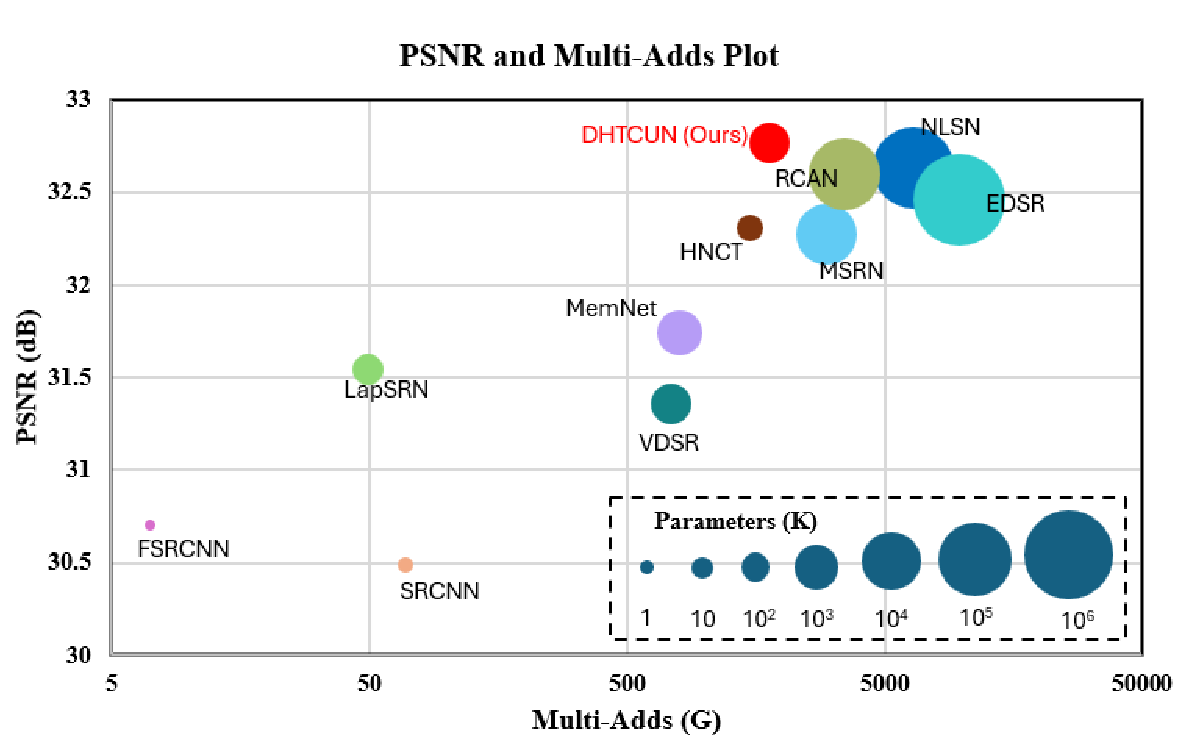
\includegraphics[width=\linewidth]{20FIGURE.pdf}
  \caption{Metric assessment of PSNR (dB) versus Multi-add where the circle size represents the number of parameters on scale factor $\times$2.}
  \label{fig:20}
\end{figure}


\subsubsection{Ablation Study by changing the number of PHTCBs in the network}

Table 2 shows the performace and computation of the model in terms of PSNR, SSIM and Multi-adds. We tried different number of Parallel Hybrid Transformer CNN Blocks (PHTBs) for our network. We trained the model for 300 epochs and compared the PSNR, SSIM and Multi-adds. The number of PHTBs showing the highest PSNR and SSIM value with lowest Multi-Adds count is chosen for the final training of the model. From Table 2 it is evident 5 PHTBs are well suited for the final model.

As such, it depends on the model's requirements. The model with four PHTBs is the best option if we need to compute less; however, if we need more performance, the model with five PHTBs is the best choice. It displays the second-lowest Multi-Adds count along with the highest PSNR and SSIM. {\color{red}\textbf{Red}} represents the optimal value, while {\color{blue}\underline{Blue}} represents the second-best value.

\begin{table}
 % \centering
  \caption{Different Number  of PHTCB in Network}
  \begin{tabular}{|c|c|c|c|c|} % Specify five columns with "c" for centered alignment
    \hline
    \textbf{Number of  PHTCB } & \textbf{Average PSNR} & \textbf{Average SSIM} & \textbf{Multi-Adds} \\
    \hline
    4   & {\color{blue}\underline{37.73}}   & {\color{blue}\underline{0.9604}}  & {\color{red}\textbf{345G}}\\
    5   & {\color{red}\textbf{37.74}}   & {\color{red}\textbf{0.9606}}   & {\color{blue}\underline{345.5G}}\\
    6   & 37.68   & 0.9600   & 348.5G\\
    7   & 37.72   & 0.9601   & 352G\\
    8   & 37.66   & 0.9598   & 353.5G\\    
    9   & 37.71   & 0.9602   & 368G\\
    10   & 37.72   & 0.9603   & 372.5G\\
% Add more rows as needed
    \hline
  \end{tabular}
\end{table}



\subsubsection{Analysing the number of ESA for the Multi-Enhanced Spatial Attention (MESA) inside the PHTCB}

We did further experiments to check the most suitable number of ESA to use in a PHTCB. The module Triple Enhanced Spatial Attention (TESA) used in PHTCB comes from Multi- Enhanced Spatial Attention (MESA). MESA employs an iterative approach in which multiple ESA are cascaded together where the output of one attention module is refined by subsequent modules, progressively enhancing the focus on critical features. The experiments included the Dual Enhanced Spatial Attention (DESA) containing two ESA modules cascaded together, Triple Enhanced Spatial Attention (TESA) consisting of three ESA modules cascaded together and Quadruple Enhanced Spatial Attention (QESA) consisting of four ESA modules cascaded together. Table 3 demonstrated that TESA can be used as MESA inside PHTCB as it gives better PSNR, SSIM and Multi-Adds count as compared to DESA or QESA on Set5 dataset.


\begin{table} 
\centering
\caption{Evaluation of MESA in the PHTCB for Set5 [42] dataset. Bold text with the color {\color{red}\textbf{Red }} indicates the best quantitative value. The {\color{blue}\underline{blue}} color and underline indicate the second best quantitative value.}

\label{table5}
\setlength{\tabcolsep}{3 pt}
\begin{tabular}{|c|c|cc|}
\hline
\multirow{2}{*}{Number of ESA in MESA} & \multirow{2}{*}{Multi-Adds} & \multicolumn{2}{c|}{Set5 [67]}  \\

\cline{3-4}&& \multicolumn{1}{c|}{PSNR}  & SSIM        \\

\hline

Dual Enhanced Spatial Attention (DESA) &{\color{red}\textbf{321G}} &\multicolumn {1}{c|}{32.84 } & 0.7808  \\

Triple Enhanced Spatial Attention (TESA) &{\color{blue}\underline{321.5G}} &\multicolumn {1}{c|}{\color{red}\textbf{34.58}} & {\color{red}\textbf{0.7848}}  \\

Quadruple Enhanced Spatial Attention (QESA) &326G &\multicolumn {1}{c|}{\color{blue}\underline{34.42}} & {\color{blue}\underline{0.7826}}  \\


\hline

\end{tabular}
\end{table}


\subsubsection{Analytical comparison with conventional denoising methods}

Here, we present a comparative analysis of our proposed DHTCUN model on the Set5 [42] Dataset for a scale factore of $\times$2 with other classical denoising techniques, including Color image denoising via sparse 3D collaborative filtering BM3D [53], Weighted Nuclear Norm Minimization with Application to Image Denoising (WNNM) [54], Denoising Convolutional Neural Network (DnCNN) [55], and Fast and Flexible Solution for CNN-Based Image Denoising (FFDNet) [56]. The Gaussian noise keeping noise level ($\sigma$) is used in Table 4 to compare performance in terms of PSNR for the values of $\sigma = 5$, $\sigma = 10$, and $\sigma = 15$. Our suggested DHTCUN model performs better at noise level $\sigma = 5$ as seen in Table 4 proving that it reduces noise amplification during the reconstruction. Thus, our model is shows better performance for noisy images too.

\begin{table*}
\centering
\caption{Assessment of image noise degradation performance on Set 5 [68] for scale factor $\times$2. Bold text with the color {\color{red}\textbf{Red }} indicates the best quantitative value. The {\color{blue}\underline{blue}} color and underline indicate the second best quantitative value.}

\label{table6}
\setlength{\tabcolsep}{2 pt}
\begin{tabular}{|c|c|c|c|c|c|c|c|} % Specify four columns with "c" for centered alignment
\hline
% {Methods} & {Factor} & {VIF}  \\
\multirow{1}{*}{Methods / Noise Level} & \multirow{1}{*}{Factor} & \multirow{1}{*}{BM3D [53]} & \multirow{1}{*}{WNNM [54]} & \multirow{1}{*}{DnCNN  [55]} & \multirow{1}{*}{FFDNet [56]}  & \multirow{1}{*}{DHTCUN (Our)}\\

\hline
$\sigma = 5$ & $\times2$  & {33.82} & {33.88} & {33.93} & {\color{blue}\underline{33.96}} & {\color{red}\textbf{33.98}}   \\
$\sigma = 10$ & $\times2$   & {32.58} & {32.64} & {32.70} & {32.75} & {32.88}   \\
$\sigma = 15$ & $\times2$  & {31.82} & {31.84} & {31.88} & {31.94} & {31.98}   \\
    
% Add more rows as needed
\hline
\end{tabular}
\end{table*}


\subsubsection{Convergence analysis}

Training convergence refers to the process by which a neural network’s learning algorithm iteratively adjusts the model parameters to minimize the loss function, thereby improving performance on a given task. Achieving training convergence is a critical aspect of developing effective deep learning models. 

We go over performance evaluation in this subsection as our model is being trained. Figure 21 displays the average PSNR (dB) for each epoch, illustrating how our model outperforms an existing SR model in terms of training convergence. To ensure a fair comparison, the training hyperparameters remain unchanged. This analysis is computed for 200 epochs of training with a ×4 enlargement factor on the DIV2K [41] dataset.


\begin{figure}
  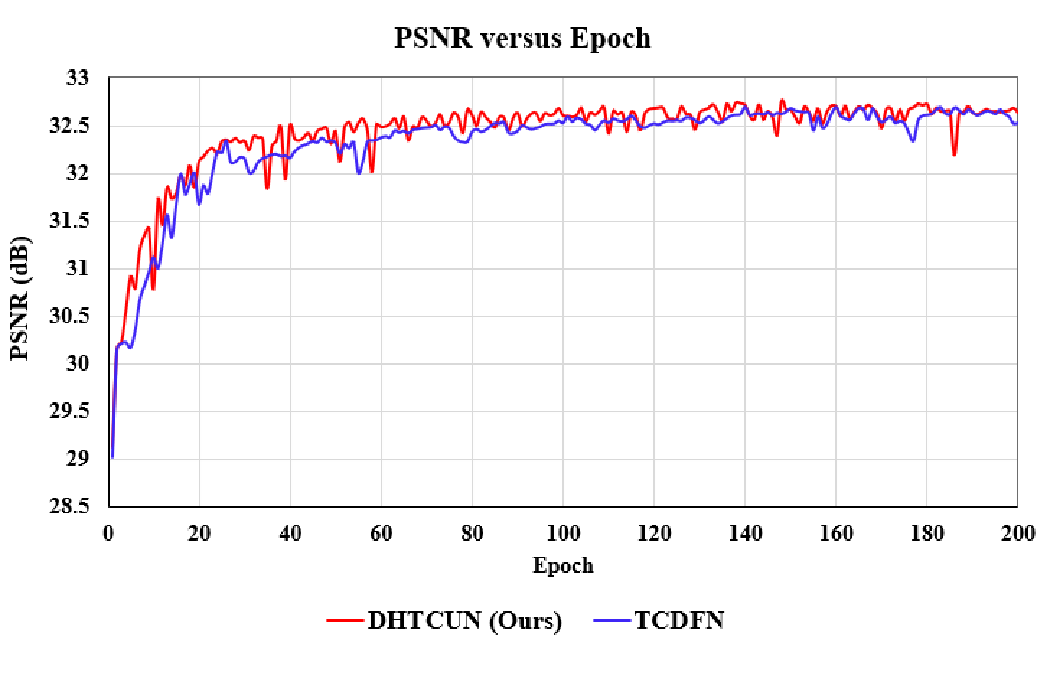
\includegraphics[width=\linewidth]{21FIGURE.pdf}
  \caption{Convergence analysis of our model with the compared to another hybrid approch.}
  \label{fig:21}
\end{figure}




\section{Discussion}

The proposed hybrid model that combines Convolutional Neural Networks (CNNs) and Transformers in a U-shaped architecture with skip connections has demonstrated notable improvements in single-image super-resolution (SISR) tasks. This novel approach leverages the complementary strengths of CNNs and Transformers to address several inherent challenges in SISR, such as computational expense, noise amplification, and the generation of artifacts like jagged patterns or blurring. By integrating the capabilities of both architectures, the model efficiently captures long-range dependencies and global context while enhancing the quality of noisy images without compromising computational efficiency.

The introduction of the Parallel Hybrid Transformer CNN Block (PHTCB) within the proposed framework stands out as a significant innovation. This block synergizes the strengths of CNNs and Transformers, enabling the model to capture intricate image details and reduce artifacts. The Transformer component excels at modeling long-range dependencies and global context, essential for reconstructing high-fidelity images from low-resolution counterparts. Concurrently, the CNN component enhances image quality, particularly in noisy scenarios, by mitigating the amplification of noise during the super-resolution process.

Furthermore, the implementation of the Triple Enhanced Spatial Attention (TESA) block contributes to the model's performance by selectively focusing on relevant image regions while suppressing irrelevant or noisy areas. This selective attention mechanism ensures that the model prioritizes crucial features, thereby improving the overall quality and perceptual realism of the super-resolved images. The TESA block's ability to enhance the model's attention to pertinent details significantly contributes to the reduction of common SISR artifacts.

In terms of computational efficiency, the proposed U-shaped backbone with skip connections plays a crucial role. This design allows the model to extract features at different levels of abstraction without substantially increasing the computational burden. The skip connections facilitate the flow of information across layers, ensuring that the model maintains a balance between capturing detailed features and preserving computational efficiency. This design choice is particularly beneficial for processing large and complex images, where computational resources are often a limiting factor.

The study's comparative analysis and experimental results support the efficacy of the suggested strategy. The model consistently outperforms the most advanced techniques in terms of perceptual quality and quantitative metrics. Especially, the suggested approach performs exceptionally well with a wide range of input image types, including extremely noisy and low-resolution images. This resilience demonstrates the model's adaptability and usefulness in real-world situations where computational effectiveness and image quality are crucial.

The proposed hybrid model represents a significant advancement in the field of SISR. By effectively combining the strengths of CNNs and Transformers within a U-shaped architecture, the model addresses several critical challenges, achieving superior image quality with reduced computational demands. The innovations introduced in the form of the PHTCB and TESA blocks further enhance the model's capabilities, making it a promising solution for high-fidelity image super-resolution tasks.


\section{Conclusions and Future Work}

In this work, we introduced a novel approach for single-image super-resolution (SISR) that synergizes the strengths of Convolutional Neural Networks (CNNs) and Transformers within a U-shaped architecture with skip connections. This hybrid model effectively addresses key challenges in SISR, including computational expense, noise amplification, and artifact generation. By leveraging the Parallel Hybrid Transformer CNN Block (PHTCB) and the Triple Enhanced Spatial Attention (TESA) block, the model captures long-range dependencies and global context while simultaneously enhancing the quality of noisy images. The U-shaped backbone with skip connections ensures efficient feature extraction at multiple levels of abstraction without increasing computational complexity. Our extensive experiments on benchmark datasets demonstrate that the proposed model consistently outperforms state-of-the-art methods in both quantitative metrics and perceptual quality. The robust performance across various image types, including those with extreme noise and low resolution, highlights the practical applicability and versatility of our approach. This work represents a significant advancement in the field of SISR, providing a promising solution for high-fidelity image reconstruction in various real-world applications. Subsequent research endeavors may delve into more refinements and expansions of this methodology, conceivably integrating supplementary attention mechanisms or sophisticated training tactics to bolster efficacy and present our model for the introduction of real-time and video super-resolution applications in intricate scenarios.






\begin{thebibliography}{00}

\bibitem{b1} Greenspan, H., \textit{Super-resolution in medical imaging}. The computer journal, 2009. 52(1): p. 43-63.

\bibitem{b2} Shakya, S., S. Kumar, and M. Goswami, \textit{Deep learning algorithm for satellite imaging based cyclone detection}. IEEE Journal of Selected Topics in Applied Earth Observations and Remote Sensing, 2020. 13: p. 827-839.

\bibitem{b3} Zhang, L., et al., \textit{A super-resolution reconstruction algorithm for surveillance images}. Signal Processing, 2010. 90(3): p. 848-859.

\bibitem{b4} Malczewski, K. and Stasiński, R. \textit{Super-resolution for multimedia, image, and video processing applications}. In Recent Advances in Multimedia Signal Processing and Communications Berlin, Heidelberg: Springer Berlin Heidelberg, 2009. pp. 171-208.

\bibitem{b5} C. Dong, C. C. Loy, K. He and X. Tang, \textit{"Image super-resolution using deep convolutional networks"}, \textit{IEEE Trans. Pattern Anal. Mach. Intell.}, vol. 38, pp. 295-307, Feb. 2015.

\bibitem{b6} Dong, C., C.C. Loy, and X. Tang. \textit{Accelerating the super-resolution convolutional neural network. in European conference on computer vision}. 2016. Springer.

\bibitem{b7} J. Kim, J. K. Lee and K. M. Lee, \textit{"Accurate image super-resolution using very deep convolutional networks"}, \textit{Proc. IEEE Conf. Comput. Vis. Pattern Recognit.}, pp. 1646-1654, Jun, 2016.

\bibitem{b8} W.-S. Lai, J.-B. Huang, N. Ahuja and M.-H. Yang, \textit{"Deep Laplacian pyramid networks for fast and accurate super-resolution"}, \textit{Proc. IEEE Conf. Comput. Vis. Pattern Recognit.}, pp. 5835-5843, Jul. 2017.

\bibitem{b9} Y. Tai, J. Yang, X. Liu and C. Xu, \textit{"MemNet: A persistent memory network for image restoration"}, \textit{Proc. IEEE Conf. Int. Conf. Comput. Vis.}, Oct 2017. pp. 4539-4547. 

\bibitem{b10} Lim, B., \textit{Enhanced deep residual networks for single image super-resolution}. in \textit{Proceedings of the IEEE conference on computer vision and pattern recognition workshops}. 2017.

\bibitem{b11} Zhang, Y., et al. \textit{Image super-resolution using very deep residual channel attention networks}. in \textit{Proceedings of the European conference on computer vision (ECCV)}. 2018.

\bibitem{b12} Mei, Y., Y. Fan, and Y. Zhou. \textit{Image super-resolution with non-local sparse attention}. in \textit{Proceedings of the IEEE/CVF Conference on Computer Vision and Pattern Recognition}. 2021.

\bibitem{b13} Talreja, J., Aramvith, S. and Onoye, T. \textit{DANS: Deep Attention Network for Single Image Super-Resolution.} IEEE Access, 2023.

\bibitem{b14} Dosovitskiy A., Beyer L., Kolesnikov A., Weissenborn D., Zhai X., Unterthiner T., Dehghani M., Minderer M., Heigold G., Gelly S., Uszkoreit J., and Houlsby N. \textit{An image is 11worth 16$\times$16 words: Transformers for image recognition at scale.} In International Conference on Learning Representations, 2021.

\bibitem{b15} Liang, J., Cao, J., Sun, G., Zhang, K., Van Gool, L. and Timofte, R. \textit{SwinIR: Image restoration using swin transformer}. In \textit{Proceedings of the IEEE/CVF international conference on computer vision}, 2021. (pp. 1833-1844).

\bibitem{b16} Liu, Z., Lin, Y., Cao, Y., Hu, H., Wei, Y., Zhang, Z., Lin, S. and Guo, B. \textit{Swin Transformer: Hierarchical vision transformer using shifted windows.} In Proceedings of the IEEE/CVF international conference on computer vision, 2021. (pp. 10012-10022).

\bibitem{b17} Zhou, Y., Li, Z., Guo, C.L., Bai, S., Cheng, M.M. and Hou, Q. \textit{SRFormer: Permuted Self-Attention for Single Image Super-Resolution.} arXiv preprint, 2023. arXiv:2303.09735.

\bibitem{b18} Zhang, X., Zeng, H., Guo, S. and Zhang, L., \textit{Efficient long-range attention network for image super-resolution.} In European Conference on Computer Vision (pp. 649-667). Cham: Springer Nature Switzerland, Oct, 2022.

\bibitem{b19} Zhou, Z., Li, G. and Wang, G., 2023. A hybrid of transformer and CNN for efficient single image super-resolution via multi-level distillation. Displays, 76, p.102352.

\bibitem{b20} Fang, J., Lin, H., Chen, X. and Zeng, K., 2022. A hybrid network of cnn and transformer for lightweight image super-resolution. In Proceedings of the IEEE/CVF conference on computer vision and pattern recognition (pp. 1103-1112).

\bibitem{b21} Zhang, W., Tan, Z., Lv, Q., Li, J., Zhu, B. and Liu, Y., 2024. An Efficient Hybrid CNN-Transformer Approach for Remote Sensing Super-Resolution. Remote Sensing, 16(5), p.880.

\bibitem{b22} Li, Z., et al. \textit{Feedback network for image super-resolution}. in \textit{Proceedings of the IEEE/CVF conference on computer vision and pattern recognition}. 2019.

\bibitem{b23} Kim, J., J.K. Lee, and K.M. Lee. \textit{Deeply-recursive convolutional network for image super-resolution}. in \textit{Proceedings of the IEEE conference on computer vision and pattern recognition}. 2016.

\bibitem{b24} Tai, Y., Yang, J. and Liu, X., \textit{Image super-resolution via deep recursive residual network}. In \textit{Proceedings of the IEEE conference on computer vision and pattern recognition}, 2017. (pp. 3147-3155).

\bibitem{b25} Li, J., Fang, F., Li, J., Mei, K. and Zhang, G., 2020. MDCN: Multi-scale dense cross network for image super-resolution. IEEE Transactions on Circuits and Systems for Video Technology, 31(7), pp.2547-2561.

\bibitem{b26} C. Ledig, L. Theis, F. Huszar, J. Caballero, A. Cunningham, A. Acosta, A. P. Aitken, A. Tejani, J. Totz, Z. Wang et al., \textit{Photorealistic single image super-resolution using a generative adversarial network} in CVPR, 2017.

\bibitem{b27} X. Wang, K. Yu, S. Wu, J. Gu, Y. Liu, C. Dong, C. C. Loy, Y. Qiao, and X. Tang, \textit{Esrgan: Enhanced super-resolution generative adversarial networks} in ECCV Workshop, 2018.

\bibitem{b28} M. S. Sajjadi, B. Scholkopf, and M. Hirsch, \textit{Enhancenet: Single image super-resolution through automated texture synthesis} in ICCV, 2017.

\bibitem{b29} Dai, T., et al. \textit{Second-order attention network for single image super-resolution}. in \textit{Proceedings of the IEEE/CVF conference on computer vision and pattern recognition}. 2019.

\bibitem{b30} Mei, Y., et al. \textit{Image super-resolution with cross-scale non-local attention and exhaustive self-exemplars mining}. in \textit{Proceedings of the IEEE/CVF conference on computer vision and pattern recognition}. 2020.

\bibitem{b31} Niu, B., Wen, W., Ren, W., Zhang, X., Yang, L., Wang, S., Zhang, K., Cao, X. and Shen, H., 2020. \textit{Single image super-resolution via a holistic attention network}. In \textit{Computer Vision–ECCV 2020: 16th European Conference, Glasgow, UK, August 23–28, 2020, Proceedings, Part XII 16} (pp. 191-207). Springer International Publishing.

\bibitem{b32} Ruangsang W., Aramvith S., and Onoye T. "Multi-FusNet of Cross Channel Network for Image Super-Resolution." IEEE Access (2023).

\bibitem{b33} Wazir M., Aramvith S., and Onoye T. \textit{"SENext: Squeeze-and-ExcitationNext for Single Image Super-Resolution." }IEEE Access (2023).

\bibitem{b34} Woo, S., Park, J., Lee, J.Y. and Kweon, I.S., 2018. Cbam: Convolutional block attention module. In Proceedings of the European conference on computer vision (ECCV) (pp. 3-19).

\bibitem{b35} Li, X., Xie, M., Zhang, Y., Ding, G. and Tong, W., 2020. Dual attention convolutional network for action recognition. IET Image Processing, 14(6), pp.1059-1065.

\bibitem{b36} Ullah, W., Hussain, T., Ullah, F.U.M., Lee, M.Y. and Baik, S.W., 2023. TransCNN: Hybrid CNN and transformer mechanism for surveillance anomaly detection. Engineering Applications of Artificial Intelligence, 123, p.106173.

\bibitem{b37} Chen, H., Wang, Y., Guo, T., Xu, C., Deng, Y., Liu, Z., Ma, S., Xu, C., Xu, C. and Gao, W., 2021. Pre-trained image processing transformer. In Proceedings of the IEEE/CVF conference on computer vision and pattern recognition (pp. 12299-12310).

\bibitem{b38} Keys, R., \textit{Cubic convolution interpolation for digital image processing}. IEEE transactions on Acoustics, speech, and signal processing, 1981. 29(6): p. 1153-1160.

\bibitem{b39} Yang, D., Li, Z., Xia, Y. and Chen, Z., 2015, July. Remote sensing image super-resolution: Challenges and approaches. In 2015 IEEE international conference on digital signal processing (DSP) (pp. 196-200). IEEE.

\bibitem{b40} Chen, Y., et al. \textit{Fsrnet: End-to-end learning face super-resolution with facial priors}. in \textit{Proceedings of the IEEE Conference on Computer Vision and Pattern Recognition}. 2018.

\bibitem{b41} Agustsson, E.,  Timofte, R. \textit{"NTIRE 2017 Challenge on Single Image Super-Resolution: Dataset and Study."} IEEE Conference on Computer Vision and Pattern Recognition Workshops (CVPRW), (2017). 126-135.

\bibitem{b42} Bevilacqua, M.; Roumy, A.; Guillemot, C.; Alberi-Morel, M.L. \textit{Low-complexity single-image super-resolution based on nonnegative neighbor embedding}. In \textit{Proceedings of the British Machine Vision Conference, Surrey}, UK, 3–7 September 2012.

\bibitem{b43} Zeyde, R.; Elad, M.; Protter, M. \textit{On Single Image Scale-Up Using Sparse-Representations}. In \textit{Proceedings of the International Conference on Curves and Surfaces}, Oslo, Norway, 28 June–3 July 2012; pp. 711–730.

\bibitem{b44} Martin, D.; Fowlkes, C.; Tal, D.; Malik, J. \textit{A database of human segmented natural images and its application to evaluating segmentation algorithms and measuring ecological statistics}. In \textit{Proceedings of the Eighth International Conference On Computer Vision} (ICCV-01), Vancouver, BC, Canada, 7–14 July 2001.

\bibitem{b45} Huang, J.-B.; Singh, A.; Ahuja, N. \textit{Single image super-resolution from transformed self-exemplars}. In \textit{Proceedings of the IEEE Conference on Computer Vision and Pattern Recognition}, Boston, MA, USA, 7–12 June 2015.

\bibitem{b46} Matsui, Y.; Ito, K.; Aramaki, Y.; Fujimoto, A.; Ogawa, T.; Yamasaki, T.; Aizawa, K. \textit{Sketch-based manga retrieval using manga109 dataset}. Multimedia. Tools Appl. 2017, 76, 21811–21838.

\bibitem{b47} Zhang, Y., et al. \textit{Residual dense network for image super-resolution}. in \textit{Proceedings of the IEEE conference on computer vision and pattern recognition}. 2018.

\bibitem{b48} J. Li, F. Fang, K. Mei and G. Zhang, \textit{"Multi-scale residual network for image super-resolution"}, \textit{Proc. Eur. Conf. Comput. Vis. (ECCV)}, Sep 2018. pp. 517-532.

\bibitem{b49} Wang, C., Li, Z. and Shi, J., \textit{Lightweight image super-resolution with adaptive weighted learning network}, 2019. arXiv preprint arXiv:1904.02

\bibitem{b50} Haris, M., Shakhnarovich, G. and Ukita, N. \textit{Deep back-projection networks for super-resolution.} In Proceedings of the IEEE conference on computer vision and pattern recognition, 2018. pp. 1664-1673.

\bibitem{b51} Zhang, Y., Tian, Y., Kong, Y., Zhong, B. and Fu, Y., 2018. Residual dense network for image super-resolution. In Proceedings of the IEEE conference on computer vision and pattern recognition (pp. 2472-2481).

\bibitem{b52} Ai, W., Tu, X., Cheng, S. and Xie, M., 2020, October. Single image super-resolution via residual neuron attention networks. In 2020 IEEE International Conference on Image Processing (ICIP) (pp. 1586-1590). IEEE.

\bibitem{b53} Dabov, K., Foi, A., Katkovnik, V. and Egiazarian, K. \textit{Color image denoising via sparse 3D collaborative filtering with grouping constraint in luminance-chrominance space.} In 2007 IEEE international conference on image processing, September 2007. (Vol. 1, pp. I-313). IEEE.

\bibitem{b54} Gu, S., Zhang, L., Zuo, W. and Feng, X. \textit{Weighted nuclear norm minimization with application to image denoising}. In Proceedings of the IEEE conference on computer vision and pattern recognition, 2014. (pp. 2862-2869).

\bibitem{b55} Chen, J. and Li, F., \textit{Denoising convolutional neural network with mask for salt and pepper noise}. IET Image Processing, 2019. 13(13), pp.2604-2613.

\bibitem{b56} Zhang, K., Zuo, W. and Zhang, L., 2018. \textit{FFDNet: Toward a fast and flexible solution for CNN-based image denoising.} IEEE Transactions on Image Processing, 27(9), pp.4608-4622.



\end{thebibliography}

\begin{IEEEbiography}[{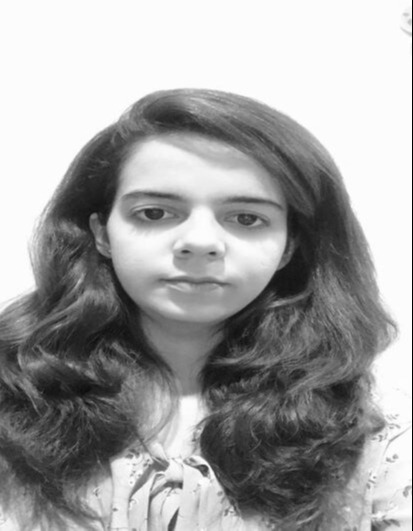
\includegraphics[width=1in,height=1.25in,clip,keepaspectratio]{a.png}}]{Jagrati Talreja} (Graduate Student Member, IEEE) received the B.TECH. in Electronics and Communication Engineering Networks from Pranveer Singh Institute of Technology, Kanpur, Uttar Pradesh, India in 2019. Ms Jagrati is pursuing her 5-year continuing doctoral degree from the Department of Electrical Engineering Chulalongkorn University Bangkok, Thailand from 2019 to 2024. Her research interests lie in Electrical Engineering, Neural Networks, and Machine Learning, specifically in Deep Learning image super-resolution.

\end{IEEEbiography}

\begin{IEEEbiography}[{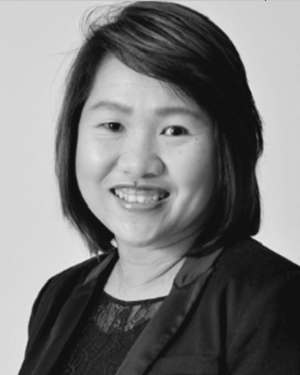
\includegraphics[width=1in,height=1.25in,clip,keepaspectratio]{b.png}}]{SUPAVADEE ARAMVITH} (Senior Member, IEEE) received the B.S. degree (Hons.) in computer science from Mahidol University, in 1993, and the M.S. and Ph.D. degrees in electrical engineering from the University of Washington, Seattle, USA, in 1996 and 2001, respectively. In June 2001, she joined Chulalongkorn University, where she is currently an Associate Professor at the Department of Electrical Engineering, specializing in video technology. She has successfully advised 32 bachelor’s, 27 master’s, and 10 Ph.D. graduates. She published over 130 articles in international conference proceedings and journals with four international book chapters. She has rich project management experiences as a project leader and a former technical committee chairs to the Thailand Government bodies in Telecommunications and ICT. She is very active in the international arena with the leadership positions in the international network such as JICA Project for AUN/SEEDNet, and the professional organizations, such as the IEEE, IEICE, APSIPA, and ITU.
\end{IEEEbiography}

\begin{IEEEbiography}[{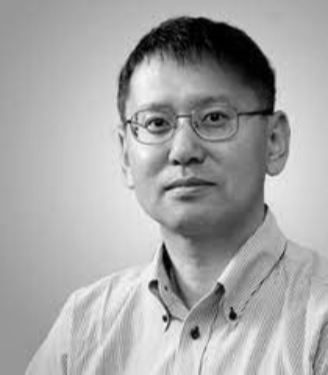
\includegraphics[width=1in,height=1.25in,clip,keepaspectratio]{c.png}}]{Takao Onoye} (Senior Member, IEEE) received the B.E. and M.E. degrees in electronic engineering and the Dr.Eng. degree in information systems engineering from Osaka University, Osaka, Japan, in 1991, 1993, and 1997, respectively. He was an Associate Professor with the Department of Communications and Computer Engineering, Kyoto University, Kyoto, Japan. Since 2003, he has been a Professor with the Department of Information Systems Engineering, Osaka University. He has published over 200 research papers in VLSI design and multimedia signal processing in reputed journals and proceedings of international conferences. His research interests include media-centric low-power architecture and its SoC implementation. Dr. Onoye has been served as a member of the CAS Society Board of Governors, since 2008. He is also a member of IEICE, IPSJ, and ITE-J.


\end{IEEEbiography}



\EOD

\end{document}
